\documentclass[a4paper,11pt]{article}

% ============================================================
%  Le Collé — Séance 1 : Déterminants, courbes paramétrées
%  © 2026 Ahmed Amine Ouqlani
% ============================================================

% ---------- Polices ----------
\usepackage[utf8]{inputenc}
\usepackage[T1]{fontenc}
\usepackage[sc]{mathpazo}          % texte et mathématiques : Palatino
\usepackage[scaled=0.88]{helvet}   % titres et repères : linéale
\linespread{1.07}
\usepackage{amsmath,amssymb,amsthm,mathrsfs,stmaryrd}
\usepackage{microtype}

% ---------- Mise en page ----------
\usepackage[a4paper,top=2.3cm,bottom=2.3cm,left=2.4cm,right=2.4cm,
            headheight=14pt,headsep=0.8cm,footskip=1.1cm]{geometry}
\setlength{\parindent}{0pt}
\setlength{\parskip}{0.45em plus 0.15em minus 0.1em}
\raggedbottom
\emergencystretch=1.5em
\clubpenalty=10000 \widowpenalty=10000 \displaywidowpenalty=10000 \brokenpenalty=10000

% ---------- Couleurs : un bleu de nuit, un ocre, des gris ----------
\usepackage{xcolor}
\definecolor{Ink}{HTML}{1C2533}
\definecolor{Bleu}{HTML}{1F3A5F}
\definecolor{BleuMoyen}{HTML}{4A6A8F}
\definecolor{BleuClair}{HTML}{9DB2C9}
\definecolor{Fond}{HTML}{F2F4F7}
\definecolor{Ocre}{HTML}{B07A26}
\definecolor{Brique}{HTML}{A23B2A}
\definecolor{Gris}{HTML}{5E6672}
\definecolor{Filet}{HTML}{C5CCD6}

% ---------- Packages ----------
\usepackage{enumitem}
\setlist{itemsep=0.25em,topsep=0.35em,parsep=0pt}
\setlist[itemize]{label=\textcolor{BleuMoyen}{\small\textbullet},leftmargin=1.4em}
\setlist[enumerate]{leftmargin=1.8em,label=\textsf{\small\color{Bleu}\arabic*.}}
\usepackage{booktabs,array,multicol}
\usepackage{needspace,float}
\usepackage[font=small,labelfont={sf,color=Bleu},labelsep=period,skip=6pt]{caption}
\usepackage{tikz}
\usetikzlibrary{arrows.meta,calc,decorations.markings}
\usepackage{pgfplots}
\pgfplotsset{compat=1.17}
\usepackage{tkz-tab}
\usepackage[most]{tcolorbox}
\usepackage{titlesec,titletoc}
\usepackage{fancyhdr,lastpage,etoolbox}
\usepackage[colorlinks=true,linkcolor=Bleu,urlcolor=Bleu,citecolor=Bleu,
            pdftitle={Le Collé — TD Courbes paramétrées (corrections)},pdfauthor={Ahmed Amine Ouqlani}]{hyperref}

\numberwithin{equation}{section}
\numberwithin{figure}{section}
\numberwithin{table}{section}

% ---------- Titres ----------
% Chapitres (sections) : grand numéro, titre en linéale, filet ocre
\titleformat{\section}[display]
  {\normalfont\sffamily\color{Ink}}
  {{\small\color{Gris}\textls[200]{\MakeUppercase{Chapitre}}}\\[-0.2em]%
   {\fontsize{64}{64}\selectfont\color{BleuClair}\thesection}}
  {0.4em}
  {\fontsize{25}{30}\selectfont\bfseries}
  [\vspace{0.5em}{\color{Ocre}\rule{3.2cm}{1.4pt}}]
\titlespacing*{\section}{0pt}{0pt}{1.6em}
\titleformat{name=\section,numberless}[display]
  {\normalfont\sffamily\color{Ink}}{}{0pt}{\fontsize{25}{30}\selectfont\bfseries}
  [\vspace{0.5em}{\color{Ocre}\rule{3.2cm}{1.4pt}}]
\titlespacing*{name=\section,numberless}{0pt}{0pt}{1.6em}

\titleformat{\subsection}
  {\needspace{5\baselineskip}\normalfont\sffamily\Large\bfseries\color{Ink}}
  {\color{Bleu}\thesubsection}{0.8em}{}
\titlespacing*{\subsection}{0pt}{1.8em}{0.5em}
\titleformat{\subsubsection}
  {\needspace{5\baselineskip}\normalfont\sffamily\large\bfseries\color{Ink}}
  {\color{Bleu}\thesubsubsection}{0.7em}{}
\titlespacing*{\subsubsection}{0pt}{1.6em}{0.4em}
\titleformat{\paragraph}[runin]{\normalfont\sffamily\bfseries\color{Ink}}{}{0pt}{}[.]
\titlespacing*{\paragraph}{0pt}{0.9em}{0.6em}
\setcounter{secnumdepth}{3}
\setcounter{tocdepth}{2}

% ---------- Table des matières ----------
\titlecontents{section}[0pt]{\addvspace{0.7em}\sffamily\bfseries\color{Ink}}
  {\makebox[2.2em][l]{\color{Bleu}\thecontentslabel}}{}{\hfill\contentspage}[\addvspace{0.2em}]
\titlecontents{subsection}[2.2em]{\small\linespread{1}\selectfont}
  {\makebox[2.6em][l]{\color{Gris}\thecontentslabel}}{}{\titlerule*[0.7pc]{.}\contentspage}

% ---------- En-têtes et pieds de page ----------
\pagestyle{fancy}
\fancyhf{}
\renewcommand{\sectionmark}[1]{\markboth{\thesection\quad#1}{}}
\fancyhead[L]{\footnotesize\sffamily\color{Gris}\leftmark}
\fancyhead[R]{\footnotesize\sffamily\scshape\color{Gris}Le Collé}
\fancyfoot[C]{\small\sffamily\color{Ink}\thepage}
\fancyfoot[L]{\scriptsize\sffamily\hyperlink{toc}{\color{Filet}sommaire}}
\renewcommand{\headrulewidth}{0.4pt}
\renewcommand{\headrule}{{\color{Filet}\hrule height\headrulewidth width\headwidth}}
\renewcommand{\footrulewidth}{0pt}
\fancypagestyle{plain}{\fancyhf{}\fancyfoot[C]{\small\sffamily\color{Ink}\thepage}\renewcommand{\headrulewidth}{0pt}}

% ---------- Énoncés ----------
\newtheoremstyle{enonce}{0pt}{0pt}{}{}{\sffamily\bfseries\color{Bleu}}{.}{0.5em}
  {\thmname{#1}\thmnumber{~#2}\thmnote{\ \normalfont\sffamily\color{Ink}(#3)}}
\newtheoremstyle{exemple}{0.9em}{0.9em}{}{}{\sffamily\bfseries\color{BleuMoyen}}{.}{0.5em}
  {\thmname{#1}\thmnumber{~#2}\thmnote{\ \normalfont\sffamily\color{Ink}(#3)}}
\newtheoremstyle{remarque}{0.7em}{0.7em}{}{}{\sffamily\itshape}{.}{0.5em}{\thmname{#1}\thmnote{\ (#3)}}
\theoremstyle{enonce}
\newtheorem{definition}{Définition}[section]
\newtheorem{theoreme}[definition]{Théorème}
\newtheorem{proposition}[definition]{Proposition}
\newtheorem{corollaire}[definition]{Corollaire}
\theoremstyle{exemple}
\newtheorem{exemple}[definition]{Exemple}
\theoremstyle{remarque}
\newtheorem*{remarque}{Remarque}

\tcbset{
  defi/.style={enhanced,breakable,colback=white,colframe=white,boxrule=0pt,arc=0pt,
     borderline west={1.2pt}{0pt}{Bleu},left=11pt,right=4pt,top=3pt,bottom=3pt,
     before skip=1.1em,after skip=1.1em},
  thm/.style={enhanced,breakable,colback=Fond,colframe=Fond,boxrule=0pt,arc=0pt,
     borderline west={2.4pt}{0pt}{Bleu},left=11pt,right=8pt,top=6pt,bottom=6pt,
     before skip=1.2em,after skip=1.2em}}
\tcolorboxenvironment{definition}{defi}
\tcolorboxenvironment{theoreme}{thm}
\tcolorboxenvironment{proposition}{thm}
\tcolorboxenvironment{corollaire}{thm}

\renewcommand{\proofname}{Démonstration}
\renewcommand{\qedsymbol}{\textcolor{BleuClair}{$\blacksquare$}}
\makeatletter
\renewenvironment{proof}[1][\proofname]{\par\pushQED{\qed}\normalfont
  \topsep0.5em\relax\trivlist\item[\hskip\labelsep\sffamily\itshape\color{Gris}#1.]\ignorespaces}
  {\popQED\endtrivlist\@endpefalse}
\makeatother

% ---------- Méthode : filets haut et bas, titre en bandeau ----------
\makeatletter\newcommand{\methlabelfix}{\protected@edef\@currentlabel{\thetcbcounter}}\makeatother
\newtcolorbox[auto counter,number within=section]{methode}[2][]{%
  enhanced,unbreakable,colback=white,colframe=white,boxrule=0pt,arc=0pt,
  borderline north={0.9pt}{0pt}{Bleu},borderline south={0.9pt}{0pt}{Bleu},
  left=4pt,right=4pt,top=8pt,bottom=8pt,before skip=1.4em,after skip=1.4em,
  before upper={\methlabelfix\phantomsection\addcontentsline{met}{metentry}{\protect\makebox[2.6em][l]{\thetcbcounter}#2}%
     {\sffamily\bfseries\small\color{white}\colorbox{Bleu}{\strut\ MÉTHODE~\thetcbcounter\ }}%
     \ \ {\sffamily\bfseries\color{Bleu}#2}\par\smallskip},#1}

% ---------- Repères pédagogiques : un filet de couleur, un mot-clé ----------
\newcommand{\definirbloc}[3]{% nom, couleur, libellé
  \newtcolorbox{#1}[1][]{enhanced,breakable,blanker,
    borderline west={1.4pt}{0pt}{#2},left=10pt,right=2pt,top=1pt,bottom=1pt,
    before skip=1em,after skip=1em,
    before upper={{\sffamily\bfseries\footnotesize\color{#2}\textls[120]{\MakeUppercase{#3}}}\quad},##1}}
\definirbloc{reflexe}{Bleu}{Réflexe}
\definirbloc{astuce}{Ocre}{Astuce}
\definirbloc{attention}{Brique}{Attention}
\definirbloc{enpratique}{BleuMoyen}{En pratique}
\definirbloc{plusloin}{Gris}{Pour aller plus loin}
\definirbloc{strategie}{Bleu}{Stratégie}
\definirbloc{lecture}{BleuMoyen}{Lire le schéma}
% compatibilité avec les parties reprises
\newenvironment{garde}{\begin{attention}}{\end{attention}}
\newenvironment{complementHP}{\begin{plusloin}}{\end{plusloin}}
\newenvironment{interpretation}{\begin{enpratique}}{\end{enpratique}}

% ---------- Exercices, corrigés ----------
\newcounter{exo}[section]
\renewcommand{\theexo}{\thesection.\arabic{exo}}
\newcommand{\niveau}[1]{{\color{Ocre}\footnotesize
  \ifcase#1\or$\bullet\circ\circ\circ\circ$\or$\bullet\bullet\circ\circ\circ$\or$\bullet\bullet\bullet\circ\circ$%
  \or$\bullet\bullet\bullet\bullet\circ$\or$\bullet\bullet\bullet\bullet\bullet$\fi}}
\newcommand{\serie}[1]{\par\needspace{8\baselineskip}\vspace{1.5em}%
  \noindent{\sffamily\bfseries\color{Bleu}#1}\par\nobreak\vspace{-0.4em}%
  \noindent{\color{Filet}\rule{\linewidth}{0.4pt}}\par\nobreak\vspace{0.1em}}
\newenvironment{exo}[3]{%
  \par\needspace{5\baselineskip}\vspace{0.75em}\refstepcounter{exo}\label{e:#1}%
  \def\exolab{#1}%
  \noindent{\sffamily\bfseries\color{Bleu}Exercice~\theexo}\quad\niveau{#2}%
  \hfill{\footnotesize\sffamily\color{Gris}#3}\par\nobreak\vspace{0.15em}}%
  {\par\nopagebreak\noindent\hfill{\scriptsize\sffamily\hyperref[c:\exolab]{\color{Gris}corrigé p.~\pageref{c:\exolab}}}\par}
\newenvironment{corrige}[1]{%
  \par\needspace{6\baselineskip}\vspace{1em}\phantomsection\label{c:#1}%
  \noindent{\sffamily\bfseries\color{Bleu}Exercice~\ref{e:#1}}\quad
  {\scriptsize\sffamily\hyperref[e:#1]{\color{Gris}énoncé p.~\pageref{e:#1}}}\par\nobreak\vspace{0.2em}}%
  {\hfill\textcolor{BleuClair}{$\square$}\par}
\newcommand{\etape}[1]{\par\smallskip\noindent{\sffamily\bfseries\small\color{BleuMoyen}#1.}\ }
\newenvironment{solution}{\par\noindent{\sffamily\bfseries\small\color{BleuMoyen}Solution.}\ }{\hfill\textcolor{BleuClair}{$\square$}\par}
\newcommand{\chercher}{\par\smallskip\noindent{\color{Filet}\rule[0.5ex]{1.2cm}{0.4pt}}\
  {\footnotesize\sffamily\itshape\color{Gris}laisser chercher l'étudiant avant de poursuivre}\par\smallskip}

% ---------- Guide de séance ----------

\newcommand{\marge}[1]{\leavevmode\marginpar{\raggedleft\scriptsize\sffamily\color{Gris}\textls[100]{\MakeUppercase{#1}}}\ignorespaces}
\newcommand{\Etape}[4]{%
  \subsection[Étape #1 --- #3 {\color{Gris}(#2)}]{#3}\label{etape:#1}%
  \noindent{\small\sffamily\color{Gris}{\color{Ocre}\bfseries Étape #1}\quad·\quad #2\quad·\quad #4}\par\medskip}
\newcommand{\question}[1]{\par\smallskip\noindent{\sffamily\bfseries\small\color{BleuMoyen}Question.}\ \textit{#1}\par\smallskip}
\newcommand{\rappel}[1]{\par\smallskip\noindent\phantomsection\addcontentsline{rap}{rapentry}{#1}%
  {\sffamily\bfseries\scriptsize\colorbox{Fond}{\color{Gris}\strut RAPPEL}}\ {\sffamily\small\color{Gris}#1.}\ }
\newcommand{\pourquoi}{\par\noindent{\sffamily\bfseries\small\color{Ocre}Pourquoi ?}\ }

% Ouverture de chapitre : \ouverture{objectifs}{prérequis}{durée}
\newcommand{\ouverture}[3]{%
  \begin{tcolorbox}[enhanced,colback=Fond,colframe=Fond,arc=0pt,boxrule=0pt,left=12pt,right=12pt,top=10pt,bottom=10pt,
     before skip=1.2em,after skip=1.6em]
  \begin{minipage}[t]{0.56\linewidth}
  {\sffamily\bfseries\small\color{Bleu}OBJECTIFS}\par\vspace{0.3em}\small #1
  \end{minipage}\hfill
  \begin{minipage}[t]{0.38\linewidth}
  {\sffamily\bfseries\small\color{Bleu}PRÉREQUIS}\par\vspace{0.3em}\small #2
  \ifx\relax#3\relax\else\par\vspace{0.6em}{\sffamily\bfseries\small\color{Bleu}DURÉE}\par\vspace{0.2em}\small #3\fi
  \end{minipage}
  \end{tcolorbox}}
% Fin de chapitre
\newenvironment{essentiel}{\par\needspace{12\baselineskip}\vspace{1.5em}%
  \begin{tcolorbox}[enhanced,unbreakable,colback=white,colframe=white,boxrule=0pt,arc=0pt,
   borderline north={1.4pt}{0pt}{Ocre},left=2pt,right=2pt,top=8pt,bottom=4pt]
  {\sffamily\bfseries\color{Ocre}L'ESSENTIEL DU CHAPITRE}\par\medskip}{\end{tcolorbox}}

% ---------- Notations ----------
\newcommand{\K}{\mathbb{K}}
\newcommand{\R}{\mathbb{R}}
\newcommand{\C}{\mathbb{C}}
\newcommand{\N}{\mathbb{N}}
\newcommand{\Z}{\mathbb{Z}}
\newcommand{\Mn}[1]{\mathcal{M}_{n}(#1)}
\newcommand{\GLn}[1]{\mathrm{GL}_n(#1)}
\newcommand{\LE}{\mathcal{L}(E)}
\newcommand{\rg}{\operatorname{rg}}
\newcommand{\vect}{\operatorname{Vect}}
\newcommand{\Mat}{\operatorname{Mat}}
\newcommand{\Id}{\operatorname{Id}}
\newcommand{\sh}{\operatorname{sh}}
\newcommand{\ch}{\operatorname{ch}}
\renewcommand{\th}{\operatorname{th}}
\DeclareMathOperator{\argsh}{argsh}
\newcommand{\vv}[1]{\overrightarrow{#1}}
\newcommand{\ve}[1]{\vec{#1}}
\newcommand{\ient}[2]{\llbracket #1,#2\rrbracket}
\newcommand{\dt}[1]{\left|\begin{matrix}#1\end{matrix}\right|}
\newcommand{\dis}{\displaystyle}

% ---------- Figures ----------
\pgfplotsset{trig format plots=rad}
\pgfplotsset{courbe/.style={axis lines=middle,axis equal image,
  axis line style={Gris,-{Stealth[length=5pt]}},
  xlabel={$x$},ylabel={$y$},ticklabel style={font=\scriptsize\sffamily,color=Gris},
  every axis x label/.style={at={(ticklabel* cs:1)},anchor=west,font=\small},
  every axis y label/.style={at={(ticklabel* cs:1)},anchor=south,font=\small},
  samples=300,smooth,width=0.6\linewidth}}
\tikzset{arcetude/.style={Bleu,line width=1.25pt},
         reste/.style={BleuClair,line width=1pt},
         tgte/.style={Ocre,line width=0.9pt},
         asy/.style={Gris,dashed,line width=0.6pt},
         pt/.style={circle,fill=Ink,inner sep=1.2pt}}

% ---------- Navigation ----------
\makeatletter
\newcommand*\l@rapentry{\@dottedtocline{1}{0em}{0em}}
\newcommand*\l@metentry{\@dottedtocline{1}{0em}{0em}}
\newcommand{\listemethodes}{\@starttoc{met}}
\newcommand{\listerappels}{\@starttoc{rap}}
\makeatother
% onglets de chapitre sur le bord droit
\usepackage{eso-pic}
\newif\ifonglets \ongletsfalse
\newcommand{\dessineronglet}{%
  \edef\ongcol{\ifnum\value{section}=3 Ocre\else Bleu\fi}%
  \edef\ongnum{\the\value{section}}%
  \pgfmathsetmacro{\ongy}{3.2+2.3*(\ongnum-1)}%
  \begin{tikzpicture}[remember picture,overlay]
  \fill[\ongcol] ([xshift=-0.75cm,yshift=-\ongy cm]current page.north east)
     rectangle ([yshift=-\ongy cm-1.9cm]current page.north east);
  \node[text=white,font=\sffamily\bfseries\large] at ([xshift=-0.37cm,yshift=-\ongy cm-0.95cm]current page.north east)
     {\ongnum};
  \end{tikzpicture}}
\AddToShipoutPictureBG{\ifonglets\ifnum\value{section}>0 \dessineronglet\fi\fi}
% blocs de navigation et d'enseignement
\definirbloc{commencer}{Gris}{Si vous commencez ici}
\definirbloc{horsprogramme}{Brique}{Hors programme}
\newcommand{\HP}{\,{\sffamily\bfseries\scriptsize\textcolor{Brique}{[HP]}}}
\newcommand{\source}[1]{{\footnotesize\sffamily\color{Gris}\,(#1)}}
\newcommand{\coupdepouce}[1]{\par\vspace{-0.2em}\noindent{\footnotesize\sffamily\color{Gris}%
  \textbf{Coup de pouce} (à donner si l'étudiant bloque) : #1}\par}
\newcommand{\pointarret}[1]{\par\vspace{1em}\noindent{\color{Filet}\rule[0.5ex]{\linewidth}{0.4pt}}\par\nobreak
  \noindent{\footnotesize\sffamily\color{Ocre}\bfseries POINT D'ARRÊT POSSIBLE}\quad{\footnotesize\sffamily\color{Gris}#1}\par\vspace{0.6em}}
\newcommand{\demarche}[1]{\noindent{\sffamily\bfseries\small\color{BleuMoyen}Démarche.}\ \textit{#1}\par\smallskip}

% ---------- Corrigés : idées, astuces, pièges, à retenir ----------
\newcommand{\choix}[1]{\par\noindent{\sffamily\bfseries\small\color{BleuMoyen}Choix de la méthode.}\ #1\par\smallskip}
\newcommand{\gain}[1]{\par\noindent{\sffamily\bfseries\small\color{Ocre}Astuce.}\ #1\par}
\newcommand{\piege}[1]{\par\noindent{\sffamily\bfseries\small\color{Brique}Piège.}\ #1\par}
\newtcolorbox{retenirbox}{enhanced,breakable,colback=Fond,colframe=Fond,arc=0pt,boxrule=0pt,
  borderline west={2pt}{0pt}{Ocre},left=8pt,right=6pt,top=4pt,bottom=4pt,before skip=0.7em,after skip=0.5em}
\newcommand{\retenir}[1]{\begin{retenirbox}{\sffamily\bfseries\footnotesize\color{Ocre}À RETENIR}\quad #1\end{retenirbox}}
\newcommand{\TD}[1]{{\color{Ocre}\bfseries TD\,#1}\ ·\ }
\newcommand{\q}[1]{\par\smallskip\noindent{\sffamily\bfseries\color{Bleu}#1}\ }
\providecommand{\iddots}{\mathinner{\mkern1mu\raise1pt\hbox{.}\mkern2mu\raise4pt\hbox{.}\mkern2mu\raise7pt\hbox{.}\mkern1mu}}

\providecommand{\Ker}{\operatorname{Ker}}\renewcommand{\Im}{\operatorname{Im}}\providecommand{\tr}{\operatorname{tr}}\providecommand{\Sp}{\operatorname{Sp}}

% ================================================================ TD : mise en page propre au livret d'exercices
\fancyhf{}
\fancyhead[L]{\footnotesize\sffamily\color{Gris}TD · Courbes paramétrées · corrections}
\fancyhead[R]{\footnotesize\sffamily\scshape\color{Gris}Le Collé}
\fancyfoot[C]{\small\sffamily\color{Ink}\thepage\,/\,\pageref{LastPage}}
\fancypagestyle{plain}{\fancyhf{}\fancyfoot[C]{\small\sffamily\color{Ink}\thepage\,/\,\pageref{LastPage}}\renewcommand{\headrulewidth}{0pt}}
\makeatletter
\newcommand{\partie}[3]{% numéro, titre, description
  \par\needspace{10\baselineskip}\vspace{1.4em}\phantomsection\label{partie:#1}\pdfbookmark[0]{Partie #1}{partie.#1}%
  {\sffamily\small\color{Gris}\textls[200]{PARTIE #1}}\par\nobreak\vspace{0.1em}
  {\sffamily\bfseries\LARGE\color{Ink}#2}\par\nobreak\vspace{0.3em}
  {\color{Ocre}\rule{2.6cm}{1.2pt}}\par\nobreak\vspace{0.2em}
  {\small\color{Gris}#3}\par\nobreak\vspace{0.6em}}
\newcommand{\exercice}[7]{% numéro, difficulté, titre, origine, notions, identifiant, page du corrigé
  \par\needspace{8\baselineskip}\vspace{1.1em}\phantomsection
  \def\@currentlabel{#1}\label{e:#6}\pdfbookmark[1]{Exercice #1}{e.#6}%
  \noindent{\sffamily\bfseries\large\color{Bleu}Exercice~#1}\quad\niveau{#2}\hfill{\footnotesize\sffamily\color{Gris}#4}\par\nobreak
  \vspace{0.1em}\noindent{\sffamily\bfseries\color{Ink}#3}\par\nobreak
  \vspace{0.1em}\noindent{\footnotesize\sffamily\color{Gris}Notions : #5.\hfill\mbox{corrigé p.~#7}\par}\nobreak
  \vspace{0.35em}}
\newcommand{\renvoi}[1]{\par\nopagebreak\vspace{0.2em}\noindent\hfill{\scriptsize\sffamily\color{Gris}#1}\par}
\newcommand{\place}{\par\vspace{1.6cm plus 0.6cm minus 0.6cm}}
\newcommand{\correction}[4]{% numéro, titre, identifiant, renvoi
  \par\needspace{7\baselineskip}\vspace{1.3em}\phantomsection
  \def\@currentlabel{#1}\label{e:#3}\pdfbookmark[1]{Exercice #1}{c.#3}%
  {\color{Filet}\hrule height 0.4pt}\vspace{0.5em}
  \noindent{\sffamily\bfseries\large\color{Bleu}Exercice~#1}\quad{\sffamily\bfseries\color{Ink}#2}\hfill{\scriptsize\sffamily\color{Gris}#4}\par\nobreak
  \vspace{0.4em}}
\newcommand{\sommaireligne}[3]{\noindent\hbox to 2.2em{\hfill\sffamily\color{Bleu}#1.}\enspace\begin{minipage}[t]{0.8\linewidth}\raggedright#2\end{minipage}\hfill\pageref{e:#3}\par}
\makeatother
\setlength{\parskip}{0.5em plus 0.15em minus 0.1em}

\begin{document}
\thispagestyle{plain}
{\sffamily\small\color{Gris}\textls[150]{LE COLLÉ · MATHÉMATIQUES PT · CHAPITRE 5}}\par\vspace{0.2em}
{\sffamily\bfseries\fontsize{26}{30}\selectfont\color{Ink}TD --- Courbes paramétrées}\par\vspace{0.3em}
{\sffamily\Large\color{BleuMoyen}Corrections}\par\vspace{0.4em}
{\color{Ocre}\rule{3.2cm}{1.4pt}}\par\vspace{0.8em}
{\small Corrections détaillées des 32 exercices du TD, dans le même ordre et avec les mêmes numéros.
Chaque correction commence par le choix de la méthode, puis détaille les calculs ; les encadrés « À retenir » résument ce qui
resservira. Les renvois « méthode~1.3 du livret » désignent le cours.
\textbf{Chercher d'abord l'exercice} avant d'ouvrir sa correction.}

\partie{I}{Applications directes du cours}{}
\correction{1}{Paramétrer des courbes usuelles}{c-param}{énoncé : TD, p.~2}
(a) $t\mapsto A+t\vv{AB}=(1+2t,\,-1+3t)$, $t\in\R$.
(b) $\theta\mapsto(2+3\cos\theta,\,-1+3\sin\theta)$, $\theta\in[0,2\pi[$.
(c) $\theta\mapsto(3\cos\theta,\,2\sin\theta)$, $\theta\in[0,2\pi[$.
(d) $t\mapsto(\ch t,\,\sh t)$, $t\in\R$ : $\ch^2t-\sh^2t=1$ et $\ch t>0$ ; réciproquement, si $x^2-y^2=1$ et $x>0$, on pose $t=\operatorname{argsh}y$, alors $x=\sqrt{1+y^2}=\ch t$.
(e) $t\mapsto(t,\ln t)$, $t>0$ (tout graphe $y=g(x)$ se paramètre par $x=t$).
\par\hfill\textcolor{BleuClair}{$\square$}\par
\correction{2}{Réduction de l'intervalle d'étude : une ellipse}{ex-ellipse}{énoncé : TD, p.~2}
$f$ est $2\pi$-périodique ; $x$ est paire et $y$ impaire : $f(-\theta)=(x,-y)$, symétrie d'axe $(Ox)$, étude sur $[0,\pi]$. Puis $f(\pi-\theta)=(-x,y)$ : symétrie d'axe $(Oy)$, étude sur $\left[0,\frac\pi2\right]$.

Sur $\left[0,\frac\pi2\right]$ : $x'=-2\sin\theta\leq0$, $y'=\cos\theta\geq0$ ; $x$ décroît de $2$ à $0$, $y$ croît de $0$ à $1$. Tangente verticale en $(2,0)$ ($f'(0)=(0,1)$), horizontale en $(0,1)$ ($f'(\frac\pi2)=(-2,0)$). Tous les points sont réguliers ($f'$ ne s'annule pas). On complète par la symétrie d'axe $(Oy)$, puis par celle d'axe $(Ox)$.

Enfin $\frac{x^2}4+y^2=\cos^2\theta+\sin^2\theta=1$ : c'est l'ellipse de demi-axes $2$ et $1$.
\retenir{un point situé sur un axe de symétrie a une tangente perpendiculaire à l'axe (sauf point stationnaire ou double).}
\par\hfill\textcolor{BleuClair}{$\square$}\par
\correction{3}{Un paramétrage rationnel du cercle}{c-cercle}{énoncé : TD, p.~2}
\q{1.} $(2t)^2+(1-t^2)^2=1+2t^2+t^4=(1+t^2)^2$, donc $x^2+y^2=1$. Avec $t=\tan\frac\theta2$ ($\theta\in\,]-\pi,\pi[$), $x=\sin\theta$ et $y=\cos\theta$ : on obtient tous les points de $\mathcal C$ sauf celui qui correspondrait à $\theta=\pi$, c'est-à-dire $(0,-1)$ (limite de $M(t)$ quand $t\to\pm\infty$). D'ailleurs $y=-1$ imposerait $1-t^2=-1-t^2$, impossible.

\q{2.} $x'(t)=\frac{2(1-t^2)}{(1+t^2)^2}$, $y'(t)=\frac{-4t}{(1+t^2)^2}$, donc $f'(1)=(0,-1)\neq\ve0$. $M(1)=(1,0)$ et la tangente est verticale : $x=1$.
\par\hfill\textcolor{BleuClair}{$\square$}\par
\correction{4}{Nature d'un point stationnaire}{c-cusp}{énoncé : TD, p.~3}
$f'(t)=(\cos t-1,\sin t)$, nul en $0$. Développements : $x=-\frac{t^3}6+o(t^3)$, $y=\frac{t^2}2+o(t^3)$, donc
\[f(t)=t^2\left(0,\tfrac12\right)+t^3\left(-\tfrac16,0\right)+o(t^3).\]
$\ve a=(0,\frac12)$ et $\ve b=(-\frac16,0)$ ne sont pas colinéaires : $p=2$, $q=3$, rebroussement de première espèce en $O$, tangente $(Oy)$.
\gain{c'est (au signe près) l'arche de cycloïde au voisinage d'un point de contact avec l'axe.}
\par\hfill\textcolor{BleuClair}{$\square$}\par
\correction{5}{Point stationnaire par développement limité}{ex-dl}{énoncé : TD, p.~3}
Avec $\sqrt{1+t}=1+\frac t2-\frac{t^2}8+\frac{t^3}{16}+o(t^3)$ et $\ln(1-t)=-t-\frac{t^2}2+o(t^2)$ :
\[x(t)=-2+\frac{t^2}4-\frac{t^3}8+o(t^3),\qquad y(t)=-t^2-\frac{t^3}2+o(t^3),\]
donc $f(t)=(-2,0)+\frac{t^2}4(1,-4)+\frac{t^3}8(-1,-4)+o(t^3)$. Il n'y a pas de terme en $t$ : $f'(0)=\ve0$, le point est stationnaire. Avec $\ve a=(1,-4)$ et $\ve b=(-1,-4)$, $\det(\ve a,\ve b)=-4-4=-8\neq0$ : $p=2$, $q=3$, \emph{rebroussement de première espèce} en $(-2,0)$, de tangente dirigée par $(1,-4)$, soit $y=-4(x+2)$.
\retenir{s'arrêter au premier vecteur non colinéaire au premier, et pas avant.}
\par\hfill\textcolor{BleuClair}{$\square$}\par
\correction{6}{Les quatre allures d'un point stationnaire}{c-pq}{énoncé : TD, p.~3}
\choix{les coordonnées sont des polynômes : le développement est exact, on lit directement les vecteurs $\ve a_p$ et $\ve a_q$.}
\begin{itemize}
\item (a) $f(t)=t^2(1,0)+t^3(0,1)$ : $p=2$ pair, $q=3$ impair, \emph{rebroussement de première espèce}, tangente $(Ox)$.
\item (b) $f(t)=t^3(1,0)+t^4(0,1)$ : $p=3$ impair, $q=4$ pair, \emph{point d'allure ordinaire} : la courbe ne rebrousse pas ($x=t^3$ change de signe avec $t$) et reste du même côté de sa tangente $(Ox)$ ($y=t^4\geq0$), comme en un point régulier qui n'est pas d'inflexion ; c'est le graphe de $y=|x|^{4/3}$.
\item (c) $f(t)=t^3(1,0)+t^5(0,1)$ : $p=3$, $q=5$ impairs, \emph{point d'inflexion} : graphe de $y=x^{5/3}$, la courbe traverse sa tangente $(Ox)$.
\item (d) $f(t)=t^2(1,0)+t^4(0,1)+t^5(0,1)$ : le premier vecteur non colinéaire à $(1,0)$ est celui de $t^4$, donc $p=2$, $q=4$ pairs, \emph{rebroussement de seconde espèce} : les deux branches ($t>0$ et $t<0$) partent dans la même direction, du même côté de la tangente $(Ox)$ ($y\approx t^4>0$), et se séparent grâce au terme $t^5$.
\end{itemize}
\retenir{$p$ = premier exposant à vecteur non nul (direction de la tangente) ; $q$ = premier exposant à vecteur non colinéaire au premier. $p$ impair : la courbe continue ; $p$ pair : elle rebrousse. $q$ impair : elle traverse sa tangente ; $q$ pair : elle reste du même côté.}
\par\hfill\textcolor{BleuClair}{$\square$}\par
\correction{7}{Inflexion : colinéarité, pas annulation}{ex-infl}{énoncé : TD, p.~3}
\q{1.} $f'=(1+2t,3t^2)$, $f''=(2,6t)$, $f''(0)=(2,0)\neq\ve0$. $\det(f',f'')=6t(1+2t)-6t^2=6t(t+1)$, qui change de signe en $0$ : $M(0)$ (régulier, $f'(0)=(1,0)$) est un point d'inflexion.

\q{2.} $g'=(1,4t^3)$, $g''=(0,12t^2)$, $g''(0)=\ve0$. $\det(g',g'')=12t^2\geq0$ ne change pas de signe : la courbe (graphe de $x\mapsto x^4$) reste au-dessus de sa tangente, pas d'inflexion.
\retenir{l'inflexion se lit sur le \emph{changement de signe} de $\det(f',f'')$, c'est-à-dire sur la colinéarité de $f'$ et $f''$.}
\par\hfill\textcolor{BleuClair}{$\square$}\par
\correction{8}{Deux asymptotes}{c-asym}{énoncé : TD, p.~4}
\q{$t\to1$.} $x$ et $y$ sont infinis ; $\frac yx=t\to1$ et $y-x=\frac{t^2-t}{t-1}=t\to1$ : asymptote $\mathcal D:y=x+1$. Position : $y-x-1=t-1$, positif si $t\to1^+$ (courbe au-dessus, $x\to+\infty$), négatif si $t\to1^-$ (au-dessous, $x\to-\infty$).

\q{$t\to\pm\infty$.} $x\to1$ et $y\to\pm\infty$ : asymptote verticale $x=1$. $x-1=\frac1{t-1}$ : la courbe est à droite quand $t\to+\infty$ ($y\to+\infty$), à gauche quand $t\to-\infty$ ($y\to-\infty$).

\emph{Contrôle.} $t=\frac x{x-1}$ et $y=tx$ : la courbe est le graphe de $y=\frac{x^2}{x-1}=x+1+\frac1{x-1}$, où l'on relit les deux asymptotes.
\par\hfill\textcolor{BleuClair}{$\square$}\par
\correction{9}{Branches infinies : asymptote et branche parabolique}{c-branches}{énoncé : TD, p.~4}
\q{1.} Quand $t\to0$, $|x|$ et $|y|$ tendent vers $+\infty$. $\frac yx=\frac{t^3+1}{t^2+1}\to1$, puis $y-x=t^2-t\to0$ : asymptote $\Delta:y=x$. Comme $y-x=t(t-1)$ : pour $t\to0^+$ (alors $x\to+\infty$), $y-x<0$, la courbe est au-dessous de $\Delta$ ; pour $t\to0^-$ ($x\to-\infty$), au-dessus.

\q{2.} Quand $t\to\pm\infty$, $x\sim t$ et $y\sim t^2$, donc $\frac yx\to\pm\infty$ : branches paraboliques de direction $(Oy)$.

\q{3.} $y-x=t(t-1)$ : la courbe est au-dessous de $\Delta$ pour $t\in\,]0,1[$, au-dessus pour $t<0$ ou $t>1$, et elle coupe $\Delta$ en un seul point, $M(1)=(2,2)$.

\q{4.} $x'(t)=\frac{t^2-1}{t^2}$ et $y'(t)=\frac{2t^3-1}{t^2}$. $x'=0$ pour $t=\pm1$, où $y'\neq0$ : tangentes verticales en $M(1)=(2,2)$ et $M(-1)=(-2,0)$.
\piege{$\lim\frac yx=1$ ne suffit pas : c'est $\lim(y-x)$ qui donne l'asymptote, et le signe de $y-x$ la position.}
\par\hfill\textcolor{BleuClair}{$\square$}\par
\correction{10}{Paramétrer une cubique par les droites issues de $O$}{c-cubique}{énoncé : TD, p.~4}
\q{1.} Si $(x,y)\in\Gamma$ et $x\neq0$, on pose $t=\frac yx$ : $t^2x^2=x^2(x+1)$, d'où $x=t^2-1$ et $y=tx=t^3-t$. Si $x=0$, alors $y=0$ : c'est $O=f(1)$. Réciproquement, $(t^3-t)^2=t^2(t^2-1)^2=x^2(x+1)$ avec $x=t^2-1$ : $f(t)\in\Gamma$. Donc $\Gamma=f(\R)$.

\q{2.} $x(-t)=x(t)$ et $y(-t)=-y(t)$ : symétrie d'axe $(Ox)$. $f(1)=f(-1)=O$ ; $f'(t)=(2t,\ 3t^2-1)$, $f'(1)=(2,2)$ et $f'(-1)=(-2,2)$ : les tangentes en $O$ sont $y=x$ et $y=-x$ (perpendiculaires).

\q{3.} $f'(0)=(0,-1)$ : tangente verticale en $M(0)=(-1,0)$. Quand $t\to\pm\infty$, $\frac yx=t\to\pm\infty$ : branches paraboliques de direction $(Oy)$. $\det(f',f'')=\dt{2t&2\\3t^2-1&6t}=12t^2-2(3t^2-1)=2(3t^2+1)>0$ : pas d'inflexion. Tracé : une boucle ($t\in[-1,1]$) d'abscisses comprises entre $-1$ et $0$, qui part de $O$, passe par $(-1,0)$ avec une tangente verticale et revient en $O$ ; puis deux branches qui s'éloignent vers la droite, l'une vers le haut, l'autre vers le bas.
\gain{une courbe algébrique ayant un point double en $O$ se paramètre en la coupant par les droites $y=tx$ : chaque droite ne la recoupe qu'en un point.}
\par\hfill\textcolor{BleuClair}{$\square$}\par
\partie{II}{Exercices classiques et méthodes incontournables}{}
\correction{11}{Tracé à partir d'un tableau}{td-c1}{énoncé : TD, p.~5}
\choix{chaque colonne du tableau est un point avec sa tangente (donnée par $(x',y')$), chaque intervalle un arc dont la
direction est donnée par les signes de $(x',y')$. Pour l'injectivité, on raisonne sur les \emph{arcs} où $x$ est monotone.}
\q{1. Points et tangentes.}
\begin{itemize}
\item $t=0$ : $O$, $f'=(-1,4)$, tangente de pente $-4$ ;
\item $t=\frac\pi3$ : $\left(-1,\frac12\right)$, $f'=(0,2)$ : tangente verticale ;
\item $t=\frac\pi2$ : $\left(-\frac12,2\right)$, $f'=(4,0)$ : tangente horizontale ;
\item $t=\frac{2\pi}3$ : $O$ à nouveau, $f'=(1,0)$ : tangente horizontale ;
\item $t=\frac{5\pi}6$ : $(2,3)$, $f'=(4,1)$ ;
\item $t\to\pi$ : $x\to+\infty$, $y\to4$ : asymptote horizontale $y=4$, la courbe est au-dessous ($y$ croît vers $4$).
\end{itemize}
Arcs : vers le haut à gauche sur $\left[0,\frac\pi3\right]$, vers le haut à droite jusqu'à $\frac\pi2$, vers le bas à droite
jusqu'à $\frac{2\pi}3$ (retour en $O$), puis vers le haut à droite.
\begin{center}
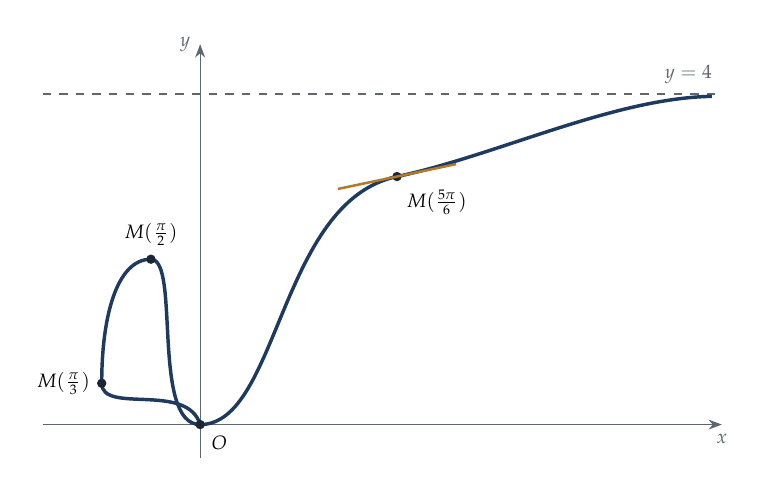
\begin{tikzpicture}[x=1.25cm,y=1.05cm,>=Stealth]
\draw[->,Gris] (-1.6,0)--(5.3,0) node[below]{\scriptsize$x$}; \draw[->,Gris] (0,-0.4)--(0,4.6) node[left]{\scriptsize$y$};
\draw[asy] (-1.6,4)--(5.3,4) node[above left]{\scriptsize$y=4$};
\draw[arcetude] (0,0) .. controls (-0.13,0.52) and (-1,0.12) .. (-1,0.5)
      .. controls (-1,1.3) and (-0.85,2) .. (-0.5,2)
      .. controls (-0.2,2) and (-0.5,0) .. (0,0)
      .. controls (0.8,0) and (0.8,2.7) .. (2,3)
      .. controls (3,3.25) and (4.2,3.95) .. (5.2,3.97);
\foreach \p in {(0,0),(-1,0.5),(-0.5,2),(2,3)} \node[pt] at \p {};
\node[font=\scriptsize,anchor=east] at (-1.02,0.5) {$M(\frac\pi3)$};
\node[font=\scriptsize,anchor=south] at (-0.5,2.05) {$M(\frac\pi2)$};
\node[font=\scriptsize,anchor=north west] at (2,2.95) {$M(\frac{5\pi}6)$};
\node[font=\scriptsize,anchor=north west] at (0.02,-0.02) {$O$};
\draw[tgte] (1.4,2.85)--(2.6,3.15);
\end{tikzpicture}
\end{center}
\q{2.} En $M\left(\frac{5\pi}6\right)=(2,3)$, $f'=(4,1)$ : $\det\big((x-2,y-3),(4,1)\big)=(x-2)-4(y-3)=0$, soit
\[x-4y+10=0\qquad\Big(y=\tfrac x4+\tfrac52\Big).\]
\q{3. Non.} Déjà $M\left(\frac{2\pi}3\right)=O$, mais $t=0$ est exclu ; il faut donc un argument plus fin. Sur
$\left]0,\frac\pi3\right]$, $x$ décroît de $0$ à $-1$ : l'arc $\Gamma_1$ est le graphe d'une fonction $h_1$ sur $[-1,0[$, à
valeurs dans $\left]0,\frac12\right]$. Sur $\left[\frac\pi3,\frac{2\pi}3\right]$, $x$ croît de $-1$ à $0$ : l'arc $\Gamma_2$ est le
graphe d'une fonction $h_2$ sur $[-1,0]$. Or :
\begin{itemize}
\item en $x=-\frac12$ : $h_2=2>\frac12\geq h_1$ ;
\item près de $0$ : $\Gamma_1$ part de $O$ avec la pente $-4$, donc $h_1(x)\sim-4x>0$ ; $\Gamma_2$ arrive en $O$ avec une tangente
      horizontale, donc $h_2(x)=o(x)$. Ainsi $h_1>h_2$ pour $x<0$ proche de $0$.
\end{itemize}
Par le théorème des valeurs intermédiaires appliqué à $h_1-h_2$ sur $\left[-\frac12,x\right]$, il existe $x_0\in\left]-\frac12,0\right[$
tel que $h_1(x_0)=h_2(x_0)$ : un point double, atteint par deux paramètres distincts de $]0,\pi]$. $g$ n'est pas injective.

\q{4. (i)} $f$ impaire : $M(-t)$ est le symétrique de $M(t)$ par rapport à $O$ (compatible avec $M(0)=O$). On ajoute l'image de
la courbe par la symétrie centrale ; la branche $t\to-\pi$ a l'asymptote $y=-4$, la courbe étant au-dessus.

\q{(ii)} $f$ $\pi$-périodique : $M(t-\pi)=M(t)$, la courbe sur $[-\pi,0[$ est parcourue une seconde fois, le dessin est le même.
Mais cette hypothèse est incompatible avec le tableau : elle imposerait $x(t)=x(t+\pi)\to+\infty$ quand $t\to0^-$, alors que $x$
est continue en $0$ avec $x(0)=0$.
\gain{pour prouver un point double sans calcul, on compare deux arcs écrits comme graphes ($x$ monotone) et l'on applique le
théorème des valeurs intermédiaires ; les pentes aux extrémités suffisent souvent.}
\piege{lire $x'(\frac\pi3)=0$ comme une tangente horizontale : c'est l'inverse ($x'=0$, $y'\neq0$ : verticale).}
\retenir{un tableau de variations conjoint contient toute l'information de tracé : points, tangentes, directions, asymptotes.
Avant d'utiliser une symétrie, vérifier sa compatibilité avec les valeurs connues.}
\par\hfill\textcolor{BleuClair}{$\square$}\par
\correction{12}{Ellipse et échelle}{td-c2}{énoncé : TD, p.~5}
\choix{lieu géométrique : on choisit le repère (le sol pour $(Ox)$, le mur pour $(Oy)$) et le paramètre imposé (l'angle) ;
« tangente » se traduit par une colinéarité, donc un déterminant nul.}
\q{1.} Soient $P$ le pied (sur $(Ox)$), $Q$ le sommet (sur $(Oy)$), $L=PQ$, et $M$ le barreau tel que $QM=a$, $MP=b$ ($L=a+b$).
Alors $P=(L\cos\theta,0)$, $Q=(0,L\sin\theta)$ et
$M=Q+\frac aL\vv{QP}=\big(a\cos\theta,(L-a)\sin\theta\big)=(a\cos\theta,b\sin\theta)$ : $M$ décrit un quart de l'ellipse
$\frac{x^2}{a^2}+\frac{y^2}{b^2}=1$ (un quart de cercle si $M$ est le milieu).

\q{2.} Valeurs pour $\theta=0,\frac\pi6,\frac\pi4,\frac\pi3,\frac\pi2$ : $(2,0)$, $\left(\sqrt3,\frac12\right)$,
$\left(\sqrt2,\frac{\sqrt2}2\right)$, $\left(1,\frac{\sqrt3}2\right)$, $(0,1)$ ; tangente verticale en $(2,0)$, horizontale en $(0,1)$.

\q{3.} L'échelle passe toujours par $M$ et est dirigée par $(\cos\theta,-\sin\theta)$ ; la courbe par
$M'(\theta)=(-a\sin\theta,b\cos\theta)\neq\ve0$. Tangence si et seulement si
\[\dt{-a\sin\theta&\cos\theta\\b\cos\theta&-\sin\theta}=a\sin^2\theta-b\cos^2\theta=0\iff\tan\theta=\sqrt{\tfrac ba}.\]
Pour $a=2$, $b=1$ : $\tan\theta=\frac1{\sqrt2}$, $\theta\approx35{,}3^\circ$, au point $M=\left(\frac{2\sqrt6}3,\frac{\sqrt3}3\right)$.
\begin{center}
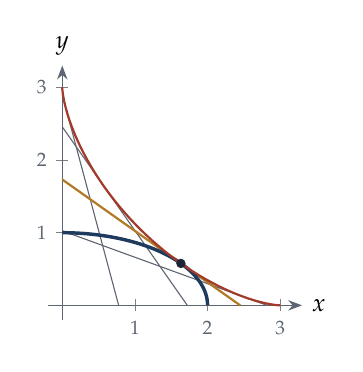
\begin{tikzpicture}
\begin{axis}[courbe,width=0.46\linewidth,xmin=-0.2,xmax=3.3,ymin=-0.2,ymax=3.3,xtick={1,2,3},ytick={1,2,3}]
\addplot[Gris,thin] coordinates {(2.819,0) (0,1.026)};
\addplot[Gris,thin] coordinates {(1.721,0) (0,2.457)};
\addplot[Gris,thin] coordinates {(0.776,0) (0,2.898)};
\addplot[Ocre,thick] coordinates {(2.449,0) (0,1.732)};
\addplot[arcetude,domain=0:1.5708,samples=100]({2*cos(x)},{sin(x)});
\addplot[Brique,thick,domain=0:1.5708,samples=100]({3*cos(x)^3},{3*sin(x)^3});
\node[pt] at (axis cs:1.633,0.577) {};
\end{axis}
\end{tikzpicture}
\end{center}
\gain{les positions de l'échelle sont toutes tangentes à l'astroïde $(L\cos^3\theta,L\sin^3\theta)$ (en brique), leur
\emph{enveloppe} (étudiée dans le volume \emph{Propriétés métriques et enveloppes}) ; la question 3 revient à chercher où l'ellipse et l'astroïde ont une tangente commune
le long de l'échelle.}
\retenir{lieu géométrique $\Rightarrow$ repère et paramètre naturels ; tangence $\Rightarrow\det(\text{vitesse},\text{direction})=0$.}
\par\hfill\textcolor{BleuClair}{$\square$}\par
\correction{13}{Symétries d'une courbe de Lissajous}{c-sym}{énoncé : TD, p.~6}
$f$ est $2\pi$-périodique : on peut se limiter à $[-\pi,\pi]$. $f(-t)=(-\sin2t,-\sin3t)=-f(t)$ : $M(-t)$ est le symétrique de $M(t)$ par rapport à $O$ ; étude sur $[0,\pi]$. Puis $f(\pi-t)=(\sin(2\pi-2t),\sin(3\pi-3t))=(-\sin2t,\sin3t)$ : symétrie d'axe $(Oy)$ ; étude sur $\left[0,\frac\pi2\right]$.

Reconstruction, dans l'ordre inverse : l'arc $\left[0,\frac\pi2\right]$, son symétrique par rapport à $(Oy)$ (arc $\left[\frac\pi2,\pi\right]$), puis le symétrique de l'ensemble par rapport à $O$ (arc $[-\pi,0]$). On remarque au passage $f(t+\pi)=(x,-y)$ : la courbe est aussi symétrique par rapport à $(Ox)$, ce qui est cohérent (centre $O$ et axe $(Oy)$ donnent l'axe $(Ox)$).
\par\hfill\textcolor{BleuClair}{$\square$}\par
\correction{14}{Points d'inflexion}{td-c6}{énoncé : TD, p.~6}
\choix{méthode~2.3 du livret : $\det(f',f'')$, factorisé, puis étude du signe. Pour les branches, $\frac yx$.}
\q{1.} $x'(t)=\frac34(t-2)^2\geq0$, $y'(t)=2t$ : pas de point stationnaire ($x'=0$ seulement en $2$, où $y'=4$).
\begin{center}
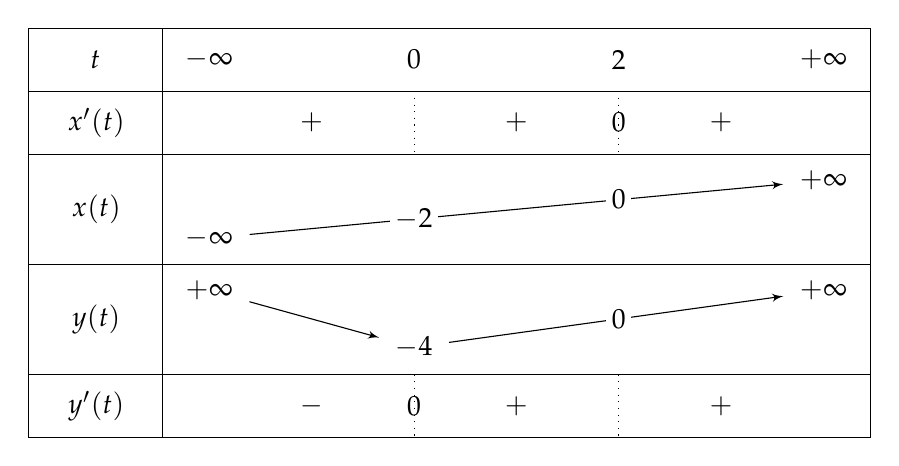
\begin{tikzpicture}
\tkzTabInit[lgt=1.7,espcl=2.6,deltacl=0.6]{$t$/0.8,$x'(t)$/0.8,$x(t)$/1.4,$y(t)$/1.4,$y'(t)$/0.8}{$-\infty$,$0$,$2$,$+\infty$}
\tkzTabLine{,+,t,+,z,+,}
\tkzTabVar{-/$-\infty$,R/,R/,+/$+\infty$}
\tkzTabIma{1}{4}{2}{$-2$}
\tkzTabIma{1}{4}{3}{$0$}
\tkzTabVar{+/$+\infty$,-/$-4$,R/,+/$+\infty$}
\tkzTabIma{2}{4}{3}{$0$}
\tkzTabLine{,-,z,+,t,+,}
\end{tikzpicture}
\end{center}
Tangente horizontale en $(-2,-4)$, verticale en $O$. Quand $t\to\pm\infty$, $\frac yx\sim\frac4t\to0$ : deux branches
paraboliques de direction $(Ox)$, \emph{aucune asymptote}.

\q{2.} $f''=\left(\frac32(t-2),2\right)$ et
\[\det(f',f'')=\frac32(t-2)^2-3t(t-2)=-\frac32(t-2)(t+2).\]
Il s'annule en $t=\pm2$ et change de signe en chacun (racines simples) : exactement deux points d'inflexion, $M(2)=O$ (tangente
verticale $x=0$) et $M(-2)=(-16,0)$, où $f'(-2)=(12,-4)$ donne la tangente $y=-\frac13(x+16)$.

\q{3.}
\begin{center}
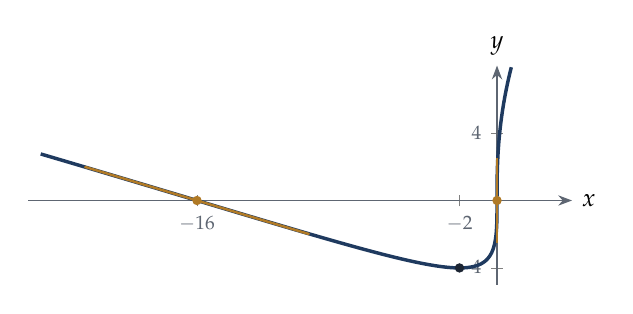
\begin{tikzpicture}
\begin{axis}[courbe,width=0.7\linewidth,height=0.36\linewidth,axis equal image=false,xmin=-25,xmax=4,ymin=-5,ymax=8,xtick={-16,-2},ytick={-4,4}]
\addplot[arcetude,domain=-2.6:3.45,samples=200]({(x-2)^3/4},{x^2-4});
\addplot[tgte,domain=-22:-10,samples=2]{-(x+16)/3};
\addplot[tgte,samples=2] coordinates {(0,-2.5) (0,2.5)};
\node[pt,fill=Ocre] at (axis cs:-16,0) {}; \node[pt,fill=Ocre] at (axis cs:0,0) {}; \node[pt] at (axis cs:-2,-4) {};
\end{axis}
\end{tikzpicture}
\end{center}
\gain{la pente $p(t)=\frac{y'}{x'}=\frac{8t}{3(t-2)^2}$ est minimale en $t=-2$ ($p=-\frac13$) : c'est l'inflexion, comme le prévoit
$p'=\frac{\det(f',f'')}{x'^2}$.}
\piege{une inflexion peut avoir une tangente verticale (ici en $O$) : elle ne se voit pas sur la pente, seulement sur le
déterminant.}
\retenir{« exactement deux » demande les deux sens : $\det=0$ (nécessaire) pour la liste des candidats, changement de signe
(suffisant) pour chacun.}
\par\hfill\textcolor{BleuClair}{$\square$}\par
\correction{15}{Position par rapport à une tangente}{c-pos}{énoncé : TD, p.~6}
\q{1.} $f'(1)=(2,3)$ et $M(1)=(1,1)$ : $3(x-1)-2(y-1)=0$, soit $T:3x-2y-1=0$.

\q{2.} On pose $\varphi(t)=3x(t)-2y(t)-1=3t^2-2t^3-1$. Comme $t=1$ est racine double (contact), on factorise : $\varphi(t)=-(t-1)^2(2t+1)$. La courbe recoupe $T$ en $t=-\frac12$, au point $\left(\frac14,-\frac18\right)$. Pour $t>-\frac12$, $\varphi(t)\leq0$ : comme $\varphi$ est du signe de $3x-2y-1$, la courbe est du côté où $3x-2y-1<0$, c'est-à-dire au-dessus de $T$ ($y>\frac{3x-1}2$) ; pour $t<-\frac12$, elle est au-dessous.
\retenir{position globale : signe de $\varphi(t)=ax(t)+by(t)+c$ ; au point de tangence, racine au moins double.}
\par\hfill\textcolor{BleuClair}{$\square$}\par
\correction{16}{Cardioïde}{td-c4}{énoncé : TD, p.~6}
\choix{dériver puis \emph{factoriser} : les dérivées sont des sommes de cosinus ou de sinus, que l'angle moitié transforme en
produits (signe immédiat).}
\q{1.} $f$ est $2\pi$-périodique, $x$ paire, $y$ impaire : axe $(Ox)$, étude sur $[0,\pi]$.

\q{2.} $e^{it}-e^{2it}=e^{\frac{3it}2}\left(e^{-\frac{it}2}-e^{\frac{it}2}\right)=-2i\sin\frac t2\,e^{\frac{3it}2}$, de partie réelle
$-2\sin\frac t2\,\mathrm{Re}\big(ie^{\frac{3it}2}\big)=2\sin\frac t2\sin\frac{3t}2$.

\q{3.} $x=\cos t-\cos^2t$ et $y=\sin t-\frac12\sin2t$, d'où
\[x'(t)=\sin t\,(2\cos t-1),\qquad y'(t)=\cos t-\cos2t=2\sin\tfrac t2\sin\tfrac{3t}2.\]
Sur $[0,\pi]$ : $x'\geq0$ sur $\left[0,\frac\pi3\right]$, $\leq0$ ensuite ; $y'>0$ sur $\left]0,\frac{2\pi}3\right[$, $<0$ ensuite.
\begin{center}
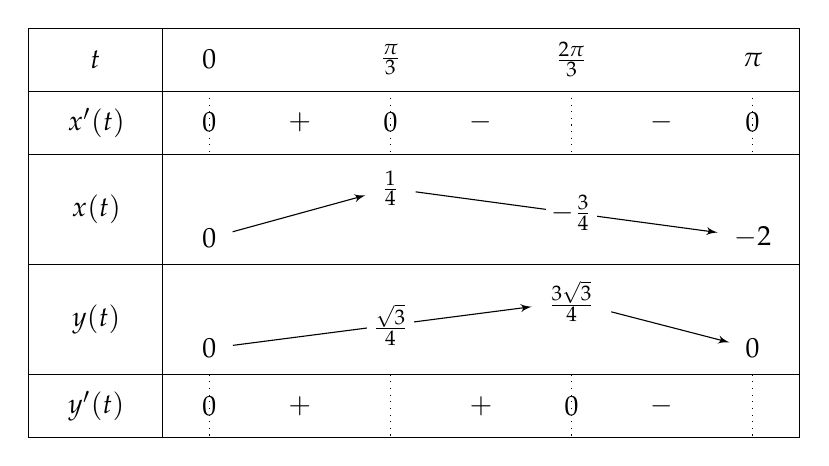
\begin{tikzpicture}
\tkzTabInit[lgt=1.7,espcl=2.3,deltacl=0.6]{$t$/0.8,$x'(t)$/0.8,$x(t)$/1.4,$y(t)$/1.4,$y'(t)$/0.8}{$0$,$\frac\pi3$,$\frac{2\pi}3$,$\pi$}
\tkzTabLine{z,+,z,-,t,-,z}
\tkzTabVar{-/$0$,+/$\frac14$,R/,-/$-2$}
\tkzTabIma{2}{4}{3}{$-\frac34$}
\tkzTabVar{-/$0$,R/,+/$\frac{3\sqrt3}4$,-/$0$}
\tkzTabIma{1}{3}{2}{$\frac{\sqrt3}4$}
\tkzTabLine{z,+,t,+,z,-,t}
\end{tikzpicture}
\end{center}
Tangente verticale en $\left(\frac14,\frac{\sqrt3}4\right)$ et en $(-2,0)$ ($f'(\pi)=(0,-2)$) ; horizontale en
$\left(-\frac34,\frac{3\sqrt3}4\right)$.

\q{4.} $f'(0)=\ve0$. Avec $1-\cos t=\frac{t^2}2+o(t^3)$ : $x=\frac{t^2}2+o(t^3)$, $y=\frac{t^2}2\cdot t+o(t^3)$, donc
$f(t)=t^2\left(\tfrac12,0\right)+t^3\left(0,\tfrac12\right)+o(t^3)$ : rebroussement de première espèce, tangente $(Ox)$, la courbe
arrivant du côté $x>0$. (À l'ordre 4, le terme $t^4\left(-\frac7{24},0\right)$ ne change rien : il est colinéaire
au premier.)

\q{5.} On place $O$ (pointe), les tangentes verticales et horizontale, on relie, puis on complète par symétrie d'axe $(Ox)$.
En polaire, $r=1-\cos\theta$ (\HP).
\begin{center}
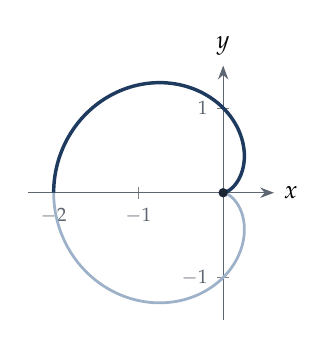
\begin{tikzpicture}
\begin{axis}[courbe,width=0.46\linewidth,xmin=-2.3,xmax=0.6,ymin=-1.5,ymax=1.5,xtick={-2,-1},ytick={-1,1}]
\addplot[reste,domain=-3.1416:0,samples=200]({(1-cos(x))*cos(x)},{(1-cos(x))*sin(x)});
\addplot[arcetude,domain=0:3.1416,samples=200]({(1-cos(x))*cos(x)},{(1-cos(x))*sin(x)});
\node[pt] at (axis cs:0,0) {};
\end{axis}
\end{tikzpicture}
\end{center}
\gain{$x'$ se factorise plus vite directement : $x'=-\sin t+2\cos t\sin t=\sin t(2\cos t-1)$. Choisir la factorisation la plus
courte, pourvu qu'elle donne le signe.}
\piege{en $t=\pi$, $x'=0$ mais $y'=-2\neq0$ : point régulier à tangente verticale, pas un point stationnaire.}
\retenir{$e^{ia}\pm e^{ib}=e^{i\frac{a+b}2}(\dots)$ : la factorisation par l'angle moitié est l'outil des dérivées
trigonométriques.}
\par\hfill\textcolor{BleuClair}{$\square$}\par
\correction{17}{Lemniscate de Bernoulli}{td-c5}{énoncé : TD, p.~7}
\choix{fractions rationnelles avec des puissances « miroirs » ($t$ et $t^3$ sur $1+t^4$) : tester $t\mapsto\frac1t$, qui échange
souvent $x$ et $y$.}
\q{Symétries.} $x\left(\frac1t\right)=\frac{1/t}{1+1/t^4}=\frac{t^3}{t^4+1}=y(t)$ et $y\left(\frac1t\right)=x(t)$ : $M(1/t)$ est le
symétrique de $M(t)$ par rapport à $y=x$, axe de symétrie. $f$ est impaire : symétrie de centre $O$. On étudie sur $[0,1]$ ;
$t\mapsto\frac1t$ donne $[1,+\infty[$, puis la symétrie centrale les $t<0$.

\q{Variations.} $x'(t)=\frac{1-3t^4}{(1+t^4)^2}$, $y'(t)=\frac{t^2(3-t^4)}{(1+t^4)^2}$. Sur $[0,1]$ : $y'\geq0$ ; $x'$ s'annule en
$t_1=3^{-1/4}\approx0{,}76$. Points : $M(0)=O$ avec $f'(0)=(1,0)$ (régulier, tangente horizontale) ;
$M(t_1)=\left(\frac34\,3^{-1/4},\frac34\,3^{-3/4}\right)\approx(0{,}57\,;0{,}33)$, tangente verticale ;
$M(1)=\left(\frac12,\frac12\right)$, $f'(1)=\left(-\frac12,\frac12\right)$ perpendiculaire à l'axe $y=x$ (point de raccord).

\q{Comportement en $\pm\infty$.} $M(t)\to O$ et $\frac yx=t^2\to+\infty$ : la courbe revient en $O$ tangentiellement à $(Oy)$
(c'est l'image par $y=x$ du départ horizontal en $t=0$). $O$ est donc un point double, de tangentes $(Ox)$ et $(Oy)$.

\q{Polaire.} $x^2+y^2=\frac{t^2(1+t^4)}{(1+t^4)^2}=\frac{t^2}{1+t^4}$ et $xy=\frac{t^4}{(1+t^4)^2}$, donc $(x^2+y^2)^2=xy$. Avec
$x=r\cos\theta$, $y=r\sin\theta$ : $r^4=r^2\cos\theta\sin\theta$, soit $r^2=\frac12\sin2\theta$ ($r\neq0$).
\begin{center}
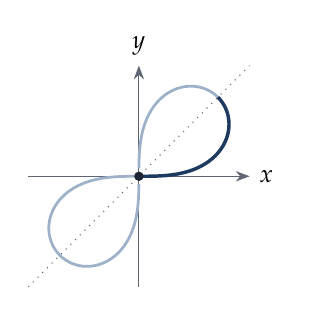
\begin{tikzpicture}
\begin{axis}[courbe,width=0.42\linewidth,xmin=-0.7,xmax=0.7,ymin=-0.7,ymax=0.7,xtick=\empty,ytick=\empty]
\addplot[Gris,dotted,domain=-0.7:0.7,samples=2]{x};
\addplot[reste,domain=-20:0,samples=600]({x/(1+x^4)},{x^3/(1+x^4)});
\addplot[reste,domain=1:20,samples=400]({x/(1+x^4)},{x^3/(1+x^4)});
\addplot[arcetude,domain=0:1,samples=100]({x/(1+x^4)},{x^3/(1+x^4)});
\node[pt] at (axis cs:0,0) {};
\end{axis}
\end{tikzpicture}
\end{center}
\piege{$O$ n'est atteint que pour $t=0$ ; le second passage est une \emph{limite} ($t\to\pm\infty$). Ne pas oublier ces limites
finies : elles ferment la courbe.}
\retenir{$t\mapsto\frac1t$ (et $t\mapsto-t$) réduisent l'étude à $[0,1]$ ; un point de l'axe de symétrie a une tangente
perpendiculaire à l'axe ; pour une équation polaire, partir de $x^2+y^2=r^2$.}
\par\hfill\textcolor{BleuClair}{$\square$}\par
\correction{18}{Cubique de Descartes}{td-c8}{énoncé : TD, p.~7}
\choix{même structure que la lemniscate (exercice~\ref{e:td-c5}) : $t\mapsto\frac1t$ échange $x$ et $y$. Pour l'asymptote : méthode~2.4 du livret
}
\q{1.} $x(1/t)=\frac{1/t}{1+1/t^3}=\frac{t^2}{t^3+1}=y(t)$ et $y(1/t)=x(t)$ : symétrie par rapport à $\Delta:y=x$. Comme $t\mapsto\frac1t$
échange $]-1,1[\setminus\{0\}$ et $]-\infty,-1[\cup]1,+\infty[$, l'étude sur $]-1,1[$ suffit.

\q{2.} $x'(t)=\frac{1-2t^3}{(1+t^3)^2}$, $y'(t)=\frac{t(2-t^3)}{(1+t^3)^2}$. Sur $]-1,1[$ : $x'$ s'annule en $t_1=2^{-1/3}$, $y'$ en
$0$. Quand $t\to-1^+$, $x\to-\infty$, $y\to+\infty$. $M(0)=O$, tangente horizontale ; $M(t_1)=\left(\frac23 2^{-1/3},\frac23 2^{-2/3}\right)
\approx(0{,}53\,;0{,}42)$, tangente verticale ; $M(1)=\left(\frac12,\frac12\right)$, tangente perpendiculaire à $\Delta$.

\q{3.} $\frac yx=t\to-1$ et $y+x=\frac{t(1+t)}{1+t^3}=\frac t{1-t+t^2}\to-\frac13$ (simplification par $1+t$) : asymptote
$\mathcal D:y=-x-\frac13$. Position :
\[y+x+\frac13=\frac{3t+1-t+t^2}{3(t^2-t+1)}=\frac{(t+1)^2}{3(t^2-t+1)}>0 :\]
la courbe est \emph{au-dessus} de $\mathcal D$, des deux côtés.
\begin{center}
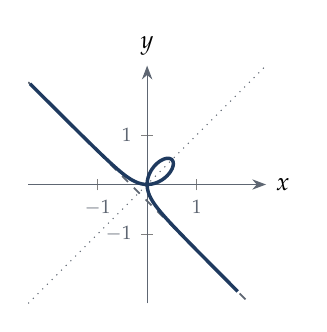
\begin{tikzpicture}
\begin{axis}[courbe,width=0.44\linewidth,xmin=-2.4,xmax=2.4,ymin=-2.4,ymax=2.4,xtick={-1,1},ytick={-1,1}]
\addplot[asy,domain=-2.4:2.4,samples=2]{-x-1/3};
\addplot[Gris,dotted,domain=-2.4:2.4,samples=2]{x};
\addplot[arcetude,domain=-0.86:40,samples=600]({x/(1+x^3)},{x^2/(1+x^3)});
\addplot[arcetude,domain=-40:-1.18,samples=300]({x/(1+x^3)},{x^2/(1+x^3)});
\end{axis}
\end{tikzpicture}
\end{center}
\gain{factoriser $1+t^3=(1+t)(1-t+t^2)$ dès le départ : la valeur interdite $-1$ et la simplification de $y+x$ apparaissent
aussitôt.}
\piege{conclure à l'asymptote avec $\frac yx\to-1$ seul : il faut $\lim(y+x)$.}
\retenir{position par rapport à une asymptote : mettre $y-(\alpha x+\beta)$ sur un dénominateur commun ; un carré au numérateur
signale que la courbe reste du même côté.}
\par\hfill\textcolor{BleuClair}{$\square$}\par
\correction{19}{Étude complète avec point double}{c-tschirn}{énoncé : TD, p.~7}
\q{1.} $x(-t)=x(t)$, $y(-t)=-y(t)$ : $M(-t)$ est le symétrique de $M(t)$ par rapport à $(Ox)$. On étudie sur $\R_+$.

\q{2.} $x'=2t\geq0$, $y'=3(t^2-1)$. $x$ croît de $0$ à $+\infty$ ; $y$ décroît de $0$ à $-2$ sur $[0,1]$, puis croît vers $+\infty$. En $t=0$ : $f'(0)=(0,-3)$, tangente verticale en $O$. En $t=1$ : $f'(1)=(2,0)$, tangente horizontale en $(1,-2)$.

\q{3.} $x(t)=x(s)$ avec $t\neq s$ impose $s=-t$ ; puis $y(t)=y(-t)$ donne $t^3-3t=0$, soit $t=\pm\sqrt3$. Le point double est $M(\sqrt3)=M(-\sqrt3)=(3,0)$. $f'(\pm\sqrt3)=(\pm2\sqrt3,6)$ : pentes $\pm\sqrt3$, droites inclinées de $\pm\frac\pi3$ sur $(Ox)$. Les tangentes font donc un angle de $\frac\pi3$ (ou $\frac{2\pi}3$).

\q{4.} Quand $t\to+\infty$ : $\frac yx\sim t\to+\infty$, branche parabolique de direction $(Oy)$. $\det(f',f'')=2t\cdot6t-3(t^2-1)\cdot2=6(t^2+1)>0$ : pas d'inflexion, la concavité ne change pas.

\q{5.} Boucle pour $t\in[-\sqrt3,\sqrt3]$, passant par $O$ (tangente verticale) et par $(1,\pm2)$ (tangentes horizontales), qui se referme en $(3,0)$ ; puis deux branches paraboliques vers le haut et vers le bas.
\par\hfill\textcolor{BleuClair}{$\square$}\par
\correction{20}{La cycloïde}{c-cycloide}{énoncé : TD, p.~8}
\q{1.} $f(t+2\pi)=f(t)+(2\pi,0)$ : la courbe est invariante par la translation de vecteur $(2\pi,0)$ ; on étudie un intervalle de longueur $2\pi$, par exemple $[-\pi,\pi]$. $f(-t)=(-x,y)$ : symétrie d'axe $(Oy)$, étude sur $[0,\pi]$. On complète par la symétrie d'axe $(Oy)$ (arche $[-\pi,\pi]$), puis par les translations de vecteurs $(2k\pi,0)$.

\q{2.} $1-\cos t=2\sin^2\frac t2$ et $\sin t=2\sin\frac t2\cos\frac t2$, d'où la factorisation. Sur $[0,\pi]$, $x'\geq0$ et $y'=\sin t\geq0$ : $x$ croît de $0$ à $\pi$, $y$ de $0$ à $2$. En $t=\pi$, $f'(\pi)=(2,0)$ : tangente horizontale au sommet $(\pi,2)$. Les points stationnaires sont les $f(2k\pi)=(2k\pi,0)$ ; la courbe $(\sin t-t,1-\cos t)$ de l'exercice~\ref{e:c-cusp} est la symétrique de la cycloïde par rapport à $(Oy)$ : ce sont des \emph{rebroussements de première espèce}, de tangente verticale.

\q{3.} Pour $t\notin2\pi\Z$, la tangente est dirigée par $\ve u=\left(\sin\frac t2,\cos\frac t2\right)$. Or
\[\vv{MH}=(\sin t,\ 1+\cos t)=2\cos\tfrac t2\left(\sin\tfrac t2,\ \cos\tfrac t2\right),\]
\[\vv{MK}=(\sin t,\ \cos t-1)=2\sin\tfrac t2\left(\cos\tfrac t2,\ -\sin\tfrac t2\right).\]
$\vv{MH}$ est colinéaire à $\ve u$ : $H$ est sur la tangente. $\vv{MK}$ est orthogonal à $\ve u$ : $K$ est sur la normale.
\gain{mécaniquement : le point de contact $K$ est immobile à l'instant considéré (roulement sans glissement), donc la vitesse de $M$ est orthogonale à $\vv{KM}$ ; c'est la construction de la tangente par le « centre instantané de rotation ».}
\par\hfill\textcolor{BleuClair}{$\square$}\par
\correction{21}{La développante du cercle}{c-develop}{énoncé : TD, p.~8}
\q{1.} $x'=-\sin t+\sin t+t\cos t=t\cos t$ et $y'=\cos t-\cos t+t\sin t=t\sin t$ : $f'(t)=t(\cos t,\sin t)$, qui ne s'annule que pour $t=0$. Seul $M(0)=(1,0)$ est stationnaire.

\q{2.} $f(t)-P(t)=(t\sin t,\ -t\cos t)$. Ce vecteur est orthogonal à $\vv{OP}=(\cos t,\sin t)$ : la droite $(PM)$ est orthogonale au rayon $[OP]$, donc tangente à $\mathcal C$ en $P$. Et $PM=t$, longueur de l'arc de cercle de rayon $1$ et d'angle $t$.

\q{3.} Pour $t>0$, la tangente en $M$ est dirigée par $(\cos t,\sin t)$, donc la normale par $(-\sin t,\cos t)$, colinéaire à $\vv{PM}$ : la normale en $M$ est la droite $(PM)$. Toutes les normales sont tangentes au cercle $\mathcal C$ : $\mathcal C$ est l'enveloppe des normales, c'est-à-dire la \emph{développée} de la courbe (volume~2).

\q{4.} $x=1-\frac{t^2}2+t^2+o(t^3)=1+\frac{t^2}2+o(t^3)$ et $y=t-\frac{t^3}6-t+\frac{t^3}2+o(t^3)=\frac{t^3}3+o(t^3)$ : $f(t)=(1,0)+t^2\left(\tfrac12,0\right)+t^3\left(0,\tfrac13\right)+o(t^3)$, avec $p=2$, $q=3$ : rebroussement de première espèce de tangente $(Ox)$ (en considérant aussi $t<0$). Enfin, avec $\ve u=(\cos t,\sin t)$ et $\ve u\,'=(-\sin t,\cos t)$ : $f'=t\ve u$, $f''=\ve u+t\ve u\,'$, donc $\det(f',f'')=\det(t\ve u,\ \ve u+t\ve u\,')=t^2\det(\ve u,\ve u\,')=t^2>0$ pour $t>0$ : pas d'inflexion.
\par\hfill\textcolor{BleuClair}{$\square$}\par
\partie{III}{Exercices de synthèse et approfondissement}{}
\correction{22}{Cissoïde de Dioclès}{td-c3}{énoncé : TD, p.~9}
\choix{suivre le plan d'étude ; pour la construction, paramétrer la droite $(OQ)$ par son angle, qui est le $\theta$ de l'énoncé.}
\q{1.} $f(\theta+\pi)=f(\theta)$ ($\sin^3$ et $\cos$ changent tous deux de signe) : période $\pi$. $x$ est impaire et $y$ paire :
$M(-\theta)$ est le symétrique de $M(\theta)$ par rapport à $(Oy)$, axe de symétrie. On étudie sur $\left[0,\frac\pi2\right[$.

\q{2.} $x'(\theta)=2a\frac{3\sin^2\theta\cos^2\theta+\sin^4\theta}{\cos^2\theta}=2a\frac{\sin^2\theta(2\cos^2\theta+1)}{\cos^2\theta}$ et
$y'(\theta)=2a\sin2\theta$. En $\frac\pi4$ : $M=(a,a)$, $f'=(4a,2a)$, direction $(2,1)$ :
$(x-a)-2(y-a)=0$, soit $T:x-2y+a=0$.

\q{3.} Sur $\left]0,\frac\pi2\right[$, $x'>0$ et $y'>0$ : $x$ croît de $0$ à $+\infty$, $y$ de $0$ à $2a$.

\q{4.} $x'=y'=0\iff\sin\theta=0$ : seul $M(0)=O$ (modulo $\pi$). À l'ordre 3 : $x=2a\theta^3+o(\theta^3)$, $y=2a\theta^2+o(\theta^3)$,
donc $f(\theta)=\theta^2(0,2a)+\theta^3(2a,0)+o(\theta^3)$ : $p=2$, $q=3$, rebroussement de première espèce en $O$, de tangente
$(Oy)$ ; la courbe est au-dessus de $O$ ($y\geq0$).

\q{5.} Quand $\theta\to\frac\pi2^-$ : $x\to+\infty$, $y\to2a$ : asymptote horizontale $\mathcal D:y=2a$. Comme $\sin^2\theta<1$, la courbe
est au-dessous. (Équation cartésienne, utile pour vérifier : $x^2(2a-y)=y^3$.)

\q{6.} $A=(0,2a)$ ; le cercle de diamètre $[OA]$ a pour équation $x^2+y^2=2ay$. Une droite issue de $O$ fait un angle $\theta$ avec
$(Oy)$ : elle est dirigée par $\ve u=(\sin\theta,\cos\theta)$. Le point $Q=r\ve u$ du cercle vérifie $r^2=2ar\cos\theta$, soit
$OQ=2a\cos\theta$ ; le point $H=r'\ve u$ de $\mathcal D$ vérifie $r'\cos\theta=2a$. D'où
\[\vv{OP}=\vv{QH}=\left(\frac{2a}{\cos\theta}-2a\cos\theta\right)\ve u=\frac{2a\sin^2\theta}{\cos\theta}(\sin\theta,\cos\theta)
=\left(2a\frac{\sin^3\theta}{\cos\theta},\,2a\sin^2\theta\right)=\vv{OM(\theta)}.\]
Quand $Q$ décrit le cercle, $\theta$ décrit $\left]-\frac\pi2,\frac\pi2\right[$ et $P$ décrit toute la cissoïde.
\begin{center}
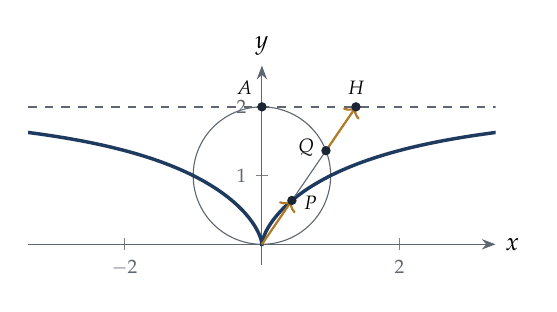
\begin{tikzpicture}
\begin{axis}[courbe,width=0.62\linewidth,xmin=-3.4,xmax=3.4,ymin=-0.3,ymax=2.6,axis equal image,xtick={-2,2},ytick={1,2}]
\addplot[asy,domain=-3.4:3.4,samples=2]{2};
\addplot[Gris,thin,domain=0:6.2832,samples=100]({cos(x)},{1+sin(x)});
\addplot[arcetude,domain=-1.13:1.13,samples=200]({2*sin(x)^3/cos(x)},{2*sin(x)^2});
\addplot[Gris] coordinates {(0,0) (1.368,2)};
\draw[->,Ocre,thick] (axis cs:0.932,1.362)--(axis cs:1.368,2);
\draw[->,Ocre,thick] (axis cs:0,0)--(axis cs:0.436,0.638);
\node[pt] at (axis cs:0.932,1.362) {}; \node[font=\scriptsize,anchor=east] at (axis cs:0.9,1.4) {$Q$};
\node[pt] at (axis cs:1.368,2) {}; \node[font=\scriptsize,anchor=south] at (axis cs:1.368,2.03) {$H$};
\node[pt] at (axis cs:0.436,0.638) {}; \node[font=\scriptsize,anchor=west] at (axis cs:0.47,0.6) {$P$};
\node[pt] at (axis cs:0,2) {}; \node[font=\scriptsize,anchor=south east] at (axis cs:0,2.03) {$A$};
\end{axis}
\end{tikzpicture}
\end{center}
\piege{l'axe de symétrie est $(Oy)$ et non $(Ox)$ : c'est $x$ qui est impaire. Ne pas plaquer le cas « usuel ».}
\gain{dans une construction issue de $O$, paramétrer chaque point par sa distance à $O$ sur la droite $O+\vect(\ve u)$ :
les équations deviennent des équations en $r$, immédiates.}
\retenir{la cissoïde réunit un rebroussement (DL à l'ordre 3), une asymptote horizontale et un lieu géométrique ; la méthode
« point courant $r\ve u$ » sert pour tous les lieux construits à partir d'un point fixe.}
\par\hfill\textcolor{BleuClair}{$\square$}\par
\correction{23}{Asymptote et prolongement}{td-c10}{énoncé : TD, p.~9}
\choix{limites de $x$ et $y$ à chaque borne : infinies $\Rightarrow$ branche (méthode~2.4 du livret) ; finies $\Rightarrow$
point limite, dont la tangente est la limite de la direction de la corde.}
\q{1.} Quand $t\to0$, $x$ et $y$ sont infinis du signe de $t$, et $\frac yx=\frac t{e^t-1}\to1$. Développement : $e^t-1=t\left(1+\frac t2+\frac{t^2}6+o(t^2)\right)$,
et $\frac1{1+u}=1-u+u^2+o(u^2)$ avec $u=\frac t2+\frac{t^2}6$ :
\[y=\frac1t\left(1-\frac t2+\frac{t^2}{12}+o(t^2)\right)=\frac1t-\frac12+\frac t{12}+o(t).\]
$y-x=-\frac12+\frac t{12}+o(t)$ : asymptote $\mathcal D:y=x-\frac12$ ; la courbe est au-dessus quand $t\to0^+$ ($x\to+\infty$),
au-dessous quand $t\to0^-$.

\q{2.} $t\to+\infty$ : $x\to0^+$, $y\sim e^{-t}\to0^+$ : $M(t)\to A=O$. Pente de la corde $\vv{AM(t)}$ : $\frac yx=\frac t{e^t-1}\to0$.
La courbe arrive en $O$ tangentiellement à $(Ox)$, par le quart de plan $x,y>0$.

\q{3.} $t\to-\infty$ : $x\to0^-$, $y\to-1$ : $M(t)\to B=(0,-1)$. $y+1=\frac{e^t}{e^t-1}<0$ et $\frac{y+1}x=\frac{te^t}{e^t-1}\to0$ :
tangente horizontale en $B$, la courbe arrivant par la gauche et par le bas.

\q{4.} $x'=-\frac1{t^2}<0$ et $y'=-\frac{e^t}{(e^t-1)^2}<0$ : sur chaque intervalle, le point va vers le bas et la gauche. Pour
$t<0$ : de $B$ (non atteint) vers $-\infty$ le long de $\mathcal D$ ; pour $t>0$ : de $+\infty$ le long de $\mathcal D$ jusqu'à $O$
(non atteint). Cohérence : avec $t=\frac1x$, le support est le graphe de $x\mapsto\frac1{e^{1/x}-1}$.
\begin{center}
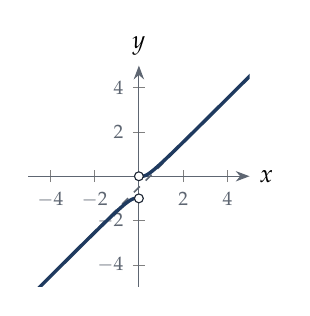
\begin{tikzpicture}
\begin{axis}[courbe,width=0.42\linewidth,xmin=-5,xmax=5,ymin=-5,ymax=5]
\addplot[asy,domain=-5:5,samples=2]{x-0.5};
\addplot[arcetude,domain=0.19:9,samples=300]({1/x},{1/(exp(x)-1)});
\addplot[arcetude,domain=-9:-0.205,samples=300]({1/x},{1/(exp(x)-1)});
\draw[Ink,fill=white] (axis cs:0,-1) circle (1.6pt);
\draw[Ink,fill=white] (axis cs:0,0) circle (1.6pt);
\end{axis}
\end{tikzpicture}
\end{center}
\gain{écrire $e^t-1=t(1+u)$ ramène le calcul à $\frac1{1+u}$ : c'est la manière la plus sûre de développer un inverse.}
\piege{oublier les bornes $t\to\pm\infty$ parce que les limites y sont finies : ce sont elles qui terminent la courbe (points
creux).}
\retenir{à chaque borne, d'abord $\lim x$ et $\lim y$ ; limite finie $\Rightarrow$ point limite et tangente $\lim\frac{y-y_A}{x-x_A}$ ;
la position se lit sur le premier terme non nul du développement asymptotique.}
\par\hfill\textcolor{BleuClair}{$\square$}\par
\correction{24}{L'astroïde}{c-astro}{énoncé : TD, p.~10}
\q{1.} $f(-t)=(x,-y)$ : axe $(Ox)$ ; $f(\pi-t)=(-x,y)$ : axe $(Oy)$ ; $f\left(\frac\pi2-t\right)=(y,x)$ : axe $y=x$. Étude sur $\left[0,\frac\pi4\right]$, puis symétries par rapport à $y=x$, $(Oy)$ et $(Ox)$.

\q{2.} $f'(t)=3\sin t\cos t\,(-\cos t,\ \sin t)$, nul pour $t\in\frac\pi2\Z$ : quatre points stationnaires $(\pm1,0)$, $(0,\pm1)$. En $0$ : $x=1-\frac32t^2+o(t^2)$, $y=t^3+o(t^3)$, donc $f(t)=(1,0)+t^2\left(-\frac32,0\right)+t^3(0,1)+o(t^3)$ : $p=2$, $q=3$, rebroussement de première espèce, tangente $(Ox)$. Par symétrie, même nature aux trois autres.

\q{3.} Pour $t\notin\frac\pi2\Z$, la tangente est dirigée par $(-\cos t,\sin t)$ :
\[\sin t\,(x-\cos^3t)+\cos t\,(y-\sin^3t)=0\iff x\sin t+y\cos t=\sin t\cos t.\]
$P=(\cos t,0)$, $Q=(0,\sin t)$, d'où $PQ=\sqrt{\cos^2t+\sin^2t}=1$ : le segment de tangente compris entre les axes a une longueur constante.
\gain{factoriser la vitesse ($f'=\lambda\ve g$) simplifie l'équation de la tangente. Le volume 2 montre la réciproque : l'astroïde est l'enveloppe d'une échelle de longueur $1$ qui glisse.}
\par\hfill\textcolor{BleuClair}{$\square$}\par
\correction{25}{La strophoïde}{c-stroph}{énoncé : TD, p.~10}
\q{1.} $x$ est paire et $y$ impaire : symétrie d'axe $(Ox)$, étude sur $\R_+$.

\q{2.} $M(1)=M(-1)=O$. $x'=\frac{4t}{(t^2+1)^2}$, $y'=\frac{t^4+4t^2-1}{(t^2+1)^2}$ : $f'(1)=(1,1)$, $f'(-1)=(-1,1)$. Les tangentes en $O$ sont $y=x$ et $y=-x$, perpendiculaires.

\q{3.} Quand $t\to\pm\infty$ : $x\to1$ et $y\to\pm\infty$ : asymptote verticale $x=1$. $x-1=-\frac2{t^2+1}<0$ : la courbe est à gauche de l'asymptote.

\q{4.} $x'=0\iff t=0$ : tangente verticale en $M(0)=(-1,0)$ (on a $y'(0)=-1\neq0$). $y'=0\iff t^4+4t^2-1=0\iff t^2=\sqrt5-2$ : tangentes horizontales aux points $\left(\frac{1-\sqrt5}2,\ \mp0{,}30\right)$ environ. Tracé : une boucle passant par $(-1,0)$, refermée en $O$, et deux branches qui longent $x=1$ par la gauche.
\par\hfill\textcolor{BleuClair}{$\square$}\par
\correction{26}{Bicorne : rebroussement de seconde espèce}{td-c7}{énoncé : TD, p.~10}
\choix{développement en $t=\frac\pi2+h$ ; il faut aller \emph{loin} (ordre 5), car le terme en $h^3$ est nul et l'on doit
trouver le premier vecteur non colinéaire au premier.}
\q{1.} $\cos t=-\sin h$, $\sin t=\cos h$. Donc $x=1-\frac{h^2}2+\frac{h^4}{24}+o(h^5)$, $\cos^2t=\sin^2h=h^2-\frac{h^4}3+o(h^5)$,
$\cos^5t=-h^5+o(h^5)$ :
\[f\left(\tfrac\pi2+h\right)=(1,0)+h^2\left(-\tfrac12,\tfrac12\right)+h^4\left(\tfrac1{24},-\tfrac16\right)+h^5(0,-1)+o(h^5).\]
$\det\big((-\frac12,\frac12),(\frac1{24},-\frac16)\big)=\frac1{12}-\frac1{48}=\frac1{16}\neq0$ : $p=2$, $q=4$, rebroussement de
\emph{seconde} espèce en $(1,0)$, tangente dirigée par $(-1,1)$ : la droite $x+y=1$. Les deux arcs sont du côté de
$\ve b=\left(\frac1{24},-\frac16\right)$ ($h^4>0$), sous cette droite.

\q{2.} $x'=\cos t$ ; $y'=-5\cos^4t\sin t-\cos t\sin t=-\sin t\cos t\,(5\cos^3t+1)$, qui s'annule pour $\cos t=-5^{-1/3}$, soit
$t=\alpha\approx2{,}20$. Symétries : $f(-t)=(-x,y)$ : axe $(Oy)$ ; étude sur $[0,\pi]$.
Signes sur $[0,\pi]$ : $x'>0$ avant $\frac\pi2$, $<0$ après ; $y'<0$ sur $\left]0,\frac\pi2\right[$, $>0$ sur $\left]\frac\pi2,\alpha\right[$,
$<0$ sur $]\alpha,\pi[$. Points : $M(0)=\left(0,\frac32\right)$ et $M(\pi)=\left(0,-\frac12\right)$, tangentes horizontales (sur l'axe) ;
$M\left(\frac\pi2\right)=(1,0)$, rebroussement ; $A=M(\alpha)$ avec $\cos\alpha=-c$, $c=5^{-1/3}$ :
$A=\left(\sqrt{1-c^2},\ c^2\left(\frac12-c^3\right)\right)=\left(\sqrt{1-c^2},\ \frac3{10}c^2\right)\approx(0{,}81\,;0{,}10)$, tangente
horizontale.

\q{3.} Sur $[0,\pi]$ : de $\left(0,\frac32\right)$ vers la droite et le bas jusqu'à la pointe $(1,0)$, retour vers la gauche et le haut
jusqu'à $A$, puis vers la gauche et le bas jusqu'à $\left(0,-\frac12\right)$ ; on complète par symétrie d'axe $(Oy)$.
\begin{center}
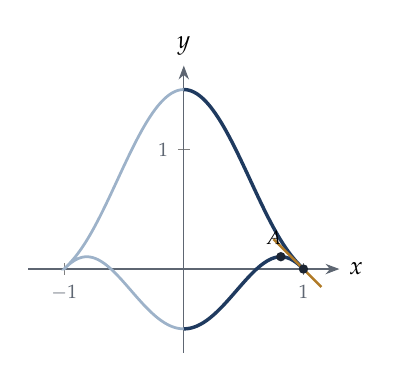
\begin{tikzpicture}
\begin{axis}[courbe,width=0.5\linewidth,xmin=-1.3,xmax=1.3,ymin=-0.7,ymax=1.7,xtick={-1,1},ytick={1}]
\addplot[reste,domain=-3.1416:0,samples=300]({sin(x)},{cos(x)^5+cos(x)^2/2});
\addplot[arcetude,domain=0:3.1416,samples=300]({sin(x)},{cos(x)^5+cos(x)^2/2});
\addplot[tgte,domain=0.75:1.15,samples=2]{1-x};
\node[pt] at (axis cs:1,0) {}; \node[pt] at (axis cs:0.811,0.103) {};
\node[font=\scriptsize,anchor=south] at (axis cs:0.75,0.12) {$A$};
\end{axis}
\end{tikzpicture}
\end{center}
\piege{s'arrêter à l'ordre 3 (aucun vecteur en $h^3$) ou à l'ordre 2 (on ne connaît que $\ve a$) : on ne peut pas conclure.
Il faut le « troisième » vecteur pour distinguer les deux espèces de rebroussement.}
\gain{$\cos^5t$ commence en $h^5$ : il est inutile de le développer plus loin, et inutile de développer $\cos^2t$ au-delà de $h^4$.}
\retenir{rebroussement de seconde espèce $\iff p$ et $q$ pairs : les deux arcs du même côté de la tangente.}
\par\hfill\textcolor{BleuClair}{$\square$}\par
\correction{27}{Axe de symétrie oblique, parabole asymptote}{td-c9}{énoncé : TD, p.~11}
\choix{la question 4 se fait en premier (elle réduit le travail) ; le point $M(1)$ est sur l'axe, et la branche
$y\sim\frac{x^2}2$ appelle une comparaison avec la parabole $y=\frac{x^2}2$.}
\q{4 (d'abord).} $x(1/t)=\frac1t+\frac{t^2}2=y(t)$ et $y(1/t)=x(t)$ : le symétrique de $M(t)$ par rapport à $y=x$ est $M(1/t)$.

\q{1.} $x'=1-\frac1{t^3}$, $y'=t-\frac1{t^2}$ s'annulent en $t=1$ : $M(1)=\left(\frac32,\frac32\right)$ stationnaire. En $t=1+h$, avec
$(1+h)^{-2}=1-2h+3h^2-4h^3+o(h^3)$ et $(1+h)^{-1}=1-h+h^2-h^3+o(h^3)$ :
\[f(1+h)=\left(\tfrac32,\tfrac32\right)+h^2\left(\tfrac32,\tfrac32\right)+h^3(-2,-1)+o(h^3),\]
$\det\big((\frac32,\frac32),(-2,-1)\big)=\frac32\neq0$ : rebroussement de première espèce, de tangente la droite $y=x$ (l'axe). Les
deux arcs partent vers le haut à droite ; $\ve b=(-2,-1)$ vérifie $y-x=1>0$ : au-dessus de l'axe pour $h>0$, au-dessous pour
$h<0$ (ils sont symétriques).

\q{2.} $x'=\frac{t^3-1}{t^3}$, $y'=\frac{t^3-1}{t^2}$. Pour $t<0$ : $x'>0$, $y'<0$ ; pour $0<t<1$ : $x'<0$, $y'<0$ ; pour $t>1$ :
$x'>0$, $y'>0$. Limites : $t\to-\infty$ : $(-\infty,+\infty)$ ; $t\to0^-$ : $(+\infty,-\infty)$ ; $t\to0^+$ : $(+\infty,+\infty)$ ;
$t\to+\infty$ : $(+\infty,+\infty)$.

\q{3.} $x^2=t^2+\frac1t+\frac1{4t^4}$, donc $y-\frac{x^2}2=\frac1t-\frac1{2t}-\frac1{8t^4}=\frac1{2t}-\frac1{8t^4}\to0$ : la parabole
$y=\frac{x^2}2$ est asymptote quand $t\to\pm\infty$ (point de même abscisse), la courbe au-dessus pour $t\to+\infty$, au-dessous
pour $t\to-\infty$. Par symétrie, quand $t\to0^\pm$, la courbe est asymptote à la parabole $x=\frac{y^2}2$.
\begin{center}
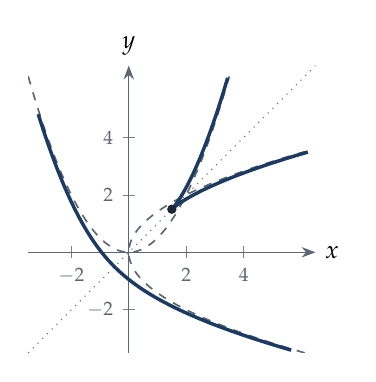
\begin{tikzpicture}
\begin{axis}[courbe,width=0.5\linewidth,xmin=-3.5,xmax=6.5,ymin=-3.5,ymax=6.5,xtick={-2,2,4},ytick={-2,2,4}]
\addplot[asy,domain=-3.5:3.5,samples=60]{x^2/2};
\addplot[asy,domain=-3.5:3.5,samples=60]({x^2/2},{x});
\addplot[Gris,dotted,domain=-3.5:6.5,samples=2]{x};
\addplot[arcetude,domain=-3.2:-0.29,samples=300]({x+1/(2*x^2)},{x^2/2+1/x});
\addplot[arcetude,domain=0.29:3.4,samples=300]({x+1/(2*x^2)},{x^2/2+1/x});
\node[pt] at (axis cs:1.5,1.5) {};
\end{axis}
\end{tikzpicture}
\end{center}
\gain{$\frac yx\to+\infty$ indique une branche parabolique de direction $(Oy)$ ; comme $y\sim\frac{t^2}2$ et $x\sim t$, on compare $y$ à
$\frac{x^2}2$ : la parabole précise la branche.}
\piege{une parabole asymptote n'est pas une asymptote au sens du programme (droite) : c'est une notion hors programme, que l'on
justifie par $M(t)P_t\to0$ avec un point $P_t$ explicite de la parabole.}
\retenir{un point stationnaire situé sur un axe de symétrie a pour tangente l'axe ou sa perpendiculaire ; les symétries
$t\mapsto\frac1t$ transforment les branches $t\to\infty$ en branches $t\to0$.}
\par\hfill\textcolor{BleuClair}{$\square$}\par
\correction{28}{Le limaçon de Pascal}{c-limacon}{énoncé : TD, p.~11}
\q{1.} $f$ est $2\pi$-périodique, $x$ paire et $y$ impaire : symétrie d'axe $(Ox)$, étude sur $[0,\pi]$.

\q{2.} $x=\cos t+2\cos^2t$, donc $x'=-\sin t-4\sin t\cos t=-\sin t(1+4\cos t)$ ; $y=\sin t+\sin2t$, donc $y'=\cos t+2\cos2t=4\cos^2t+\cos t-2$. Les racines de $4X^2+X-2$ sont $c_\pm=\frac{-1\pm\sqrt{33}}8$ ; on note $t_1=\arccos c_+\approx0{,}94$, $t_2=\arccos\left(-\frac14\right)\approx1{,}82$ et $t_3=\arccos c_-\approx2{,}57$.
\begin{center}
\renewcommand{\arraystretch}{1.25}
\begin{tabular}{c|ccccccccccc}
$t$ & $0$ & & $t_1$ & & $t_2$ & & $\frac{2\pi}3$ & & $t_3$ & & $\pi$\\\hline
$x'$ & $0$ & $-$ & & $-$ & $0$ & $+$ & & $+$ & & $+$ & $0$\\
$x$ & $3$ & $\searrow$ & $\approx1{,}30$ & $\searrow$ & $-\frac18$ & $\nearrow$ & $0$ & $\nearrow$ & $\approx0{,}58$ & $\nearrow$ & $1$\\
$y'$ & $3$ & $+$ & $0$ & $-$ & & $-$ & & $-$ & $0$ & $+$ & $1$\\
$y$ & $0$ & $\nearrow$ & $\approx1{,}76$ & $\searrow$ & $\frac{\sqrt{15}}8$ & $\searrow$ & $0$ & $\searrow$ & $\approx-0{,}37$ & $\nearrow$ & $0$
\end{tabular}
\end{center}
Tangentes verticales en $(3,0)$, $\left(-\frac18,\frac{\sqrt{15}}8\right)$ et $(1,0)$ ; horizontales en $M(t_1)\approx(1{,}30\,;1{,}76)$ et $M(t_3)\approx(0{,}58\,;-0{,}37)$. La courbe est régulière ($x'$ et $y'$ ne s'annulent jamais ensemble).

\q{3.} $M(t)=O\iff1+2\cos t=0\iff t=\pm\frac{2\pi}3$ ($[2\pi]$). $f'\left(\frac{2\pi}3\right)=\left(\frac{\sqrt3}2,-\frac32\right)$, de pente $-\sqrt3$ ; par symétrie, $f'\left(-\frac{2\pi}3\right)=\left(\frac{\sqrt3}2,\frac32\right)$, de pente $\sqrt3$. Les tangentes en $O$ font avec $(Ox)$ les angles $\mp\frac\pi3$ : elles forment un angle de $\frac\pi3$.

\q{4.} Le calcul (utiliser $\cos^2+\sin^2=1$) donne $\det(f',f'')=9+6\cos t=3(3+2\cos t)>0$ : la courbe n'a pas de point d'inflexion. Tracé : une grande boucle extérieure ($t\in\left[-\frac{2\pi}3,\frac{2\pi}3\right]$) passant par $(3,0)$, et une petite boucle intérieure ($t\in\left[\frac{2\pi}3,\frac{4\pi}3\right]$) passant par $(1,0)$, toutes deux issues de $O$.
\gain{en notant $r(t)=1+2\cos t$, $f(t)=r(t)(\cos t,\sin t)$ : $O$ est atteint exactement quand $r$ s'annule.}
\par\hfill\textcolor{BleuClair}{$\square$}\par
\correction{29}{Une courbe de Lissajous : synthèse}{ex-liss}{énoncé : TD, p.~11}
\q{Réduction.} $f$ est $2\pi$-périodique ; $f(-t)=(x,-y)$ : axe $(Ox)$ ; $f(\pi-t)=(-x,y)$ : axe $(Oy)$. Étude sur
$\left[0,\frac\pi2\right]$ : $x'=-3\sin3t$ (nul en $0$, $\frac\pi3$), $y'=2\cos t>0$ sauf en $\frac\pi2$ : courbe régulière.
$x$ : $1\searrow-1$ ($t=\frac\pi3$) $\nearrow0$ ; $y$ : $0\nearrow2$. Tangentes verticales en $(1,0)$ et $(-1,\sqrt3)$,
horizontale en $(0,2)$.

\q{Point double.} $M\left(\frac\pi6\right)=M\left(\frac{5\pi}6\right)=(0,1)=J$, avec $f'\left(\frac\pi6\right)=(-3,\sqrt3)$ et
$f'\left(\frac{5\pi}6\right)=(-3,-\sqrt3)$ : $T_1:y=-\frac x{\sqrt3}+1$, $T_2:y=\frac x{\sqrt3}+1$.

\q{Intersection de $T_2$ et de la courbe.} $M(t)\in T_2\iff2\sin t=\frac{\cos3t}{\sqrt3}+1$. On pose $X=\cos t$ :
$\cos3t=4X^3-3X$ (partie réelle de $(\cos t+i\sin t)^3$), d'où $2\sqrt3\sin t=4X^3-3X+\sqrt3$. On élève au carré
($\sin^2t=1-X^2$) :
\[P(X)=(4X^3-3X+\sqrt3)^2-12(1-X^2)=16\left(X-\tfrac{\sqrt3}2\right)\left(X+\tfrac{\sqrt3}2\right)^2\left(X^3-\tfrac{\sqrt3}2X^2+\tfrac{\sqrt3}2\right).\]
La racine double $-\frac{\sqrt3}2$ correspond à la tangence ($t=\frac{5\pi}6$), la racine simple $\frac{\sqrt3}2$ au passage de
l'autre branche par $J$ ($t=\frac\pi6$) ; le dernier facteur a une racine réelle $X_0\approx-0{,}735$, pour laquelle
$\sin t=\frac{4X_0^3-3X_0+\sqrt3}{2\sqrt3}\approx0{,}68>0$ (vérification du signe, indispensable après une élévation au
carré). $T_2$ recoupe donc la courbe en un seul autre point, $K\approx(0{,}62\,;1{,}36)$.

\q{Inflexions.} $\det(f',f'')=\dt{-3\sin3t&-9\cos3t\\2\cos t&-2\sin t}=6(\sin3t\sin t+3\cos3t\cos t)$. En posant $u=\tan t$ :
$\tan t\tan3t=-3\iff u^4+6u^2-3=0\iff u^2=2\sqrt3-3$. Plus court : on linéarise,
$\det=12\cos2t+6\cos4t=6(2c^2+2c-1)$ avec $c=\cos2t$, nul pour $c=\frac{\sqrt3-1}2$. Sur $\left[0,\frac\pi2\right]$, une seule
solution $\alpha=\arctan\sqrt{2\sqrt3-3}\approx0{,}598$, où le déterminant change de signe : $M(\alpha)\approx(-0{,}22\,;1{,}13)$
est un point d'inflexion (autre vérification : $\det(f'(\alpha),f'''(\alpha))=-48\sin3\alpha\cos\alpha\neq0$, d'où $q=3$). Par
symétrie, quatre inflexions.

\begin{figure}[h!]
\centering
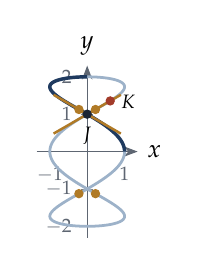
\begin{tikzpicture}
\begin{axis}[courbe,width=0.36\linewidth,xmin=-1.35,xmax=1.35,ymin=-2.3,ymax=2.3,xtick={-1,1},ytick={-2,-1,1,2}]
\addplot[reste,domain=0:6.2832,samples=400]({cos(3*x)},{2*sin(x)});
\addplot[arcetude,domain=0:1.5708,samples=200]({cos(3*x)},{2*sin(x)});
\addplot[tgte,domain=-0.9:0.9,samples=2]{-x/sqrt(3)+1};
\addplot[tgte,domain=-0.9:0.9,samples=2]{x/sqrt(3)+1};
\node[pt] at (axis cs:0,1) {}; \node[font=\scriptsize,anchor=north] at (axis cs:0,0.92) {$J$};
\node[pt,fill=Brique] at (axis cs:0.6154,1.3553) {}; \node[font=\scriptsize,anchor=west] at (axis cs:0.65,1.33) {$K$};
\node[pt,fill=Ocre] at (axis cs:-0.2214,1.126) {}; \node[pt,fill=Ocre] at (axis cs:0.2214,1.126) {};
\node[pt,fill=Ocre] at (axis cs:-0.2214,-1.126) {}; \node[pt,fill=Ocre] at (axis cs:0.2214,-1.126) {};
\end{axis}
\end{tikzpicture}
\caption{La courbe $(\cos3t,2\sin t)$ ; trait plein : arc $\left[0,\frac\pi2\right]$ ; en ocre, les tangentes en $J$ et les
inflexions ; en brique, le point $K$ où $T_2$ recoupe la courbe.}
\end{figure}
\par\hfill\textcolor{BleuClair}{$\square$}\par
\partie{IV}{Exercices difficiles et type concours}{}
\correction{30}{Problème type devoir surveillé}{ds-pb}{énoncé : TD, p.~12}
\choix{chaque question réinvestit une méthode du livre (factorisation des dérivées, développement en $t_0\neq0$, position globale, asymptotes, courbe asymptote, inflexion par factorisation de la vitesse). On note les valeurs interdites dès le début : $-3$ (borne) et $0$.}

\textbf{1.(a)} $x'(t)=-\frac4{t^2}+\frac1{t+3}=\frac{t^2-4t-12}{t^2(t+3)}=\frac{(t-6)(t+2)}{t^2(t+3)}$ et
$y'(t)=1-\frac4{t^2}=\frac{(t-2)(t+2)}{t^2}$. Comme $t^2>0$ et $t+3>0$, les signes se lisent sur les facteurs affines. Limites et
valeurs : $x\to-\infty$, $y\to-\frac{13}3$ quand $t\to-3$ ; $M(-2)=(-2,-4)$ ($\ln1=0$) ; $x,y\to-\infty$ quand $t\to0^-$ et
$+\infty$ quand $t\to0^+$ ; $M(2)=(2+\ln5,\,4)$ ; $M(6)=\left(\frac23+\ln9,\,\frac{20}3\right)$ ; $x,y\to+\infty$ quand $t\to+\infty$.
\begin{center}
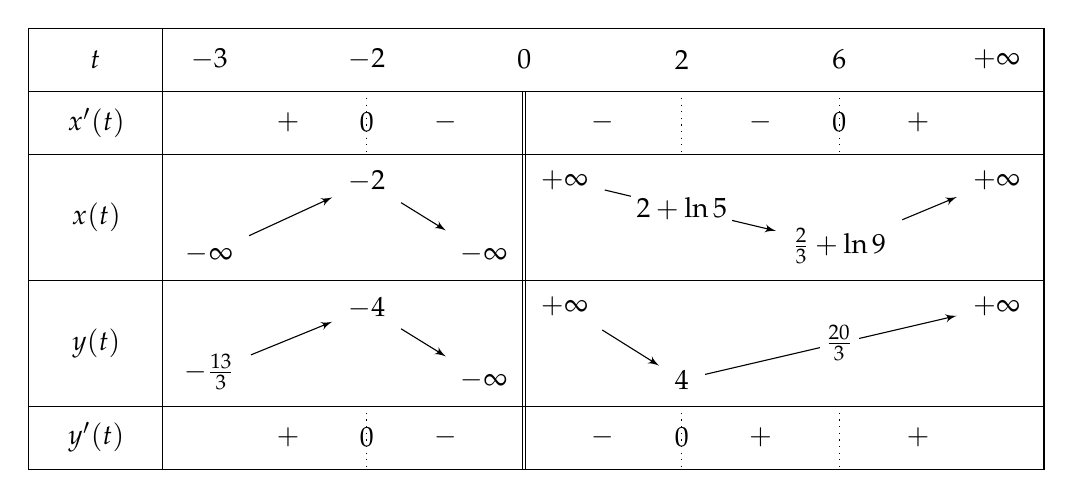
\begin{tikzpicture}
\tkzTabInit[lgt=1.7,espcl=2,deltacl=0.6]{$t$/0.8,$x'(t)$/0.8,$x(t)$/1.6,$y(t)$/1.6,$y'(t)$/0.8}{$-3$,$-2$,$0$,$2$,$6$,$+\infty$}
\tkzTabLine{,+,z,-,d,-,t,-,z,+,}
\tkzTabVar{-/$-\infty$,+/$-2$,-D+/$-\infty$/$+\infty$,R/,-/$\frac23+\ln9$,+/$+\infty$}
\tkzTabIma{3}{5}{4}{$2+\ln5$}
\tkzTabVar{-/$-\frac{13}3$,+/$-4$,-D+/$-\infty$/$+\infty$,-/$4$,R/,+/$+\infty$}
\tkzTabIma{4}{6}{5}{$\frac{20}3$}
\tkzTabLine{,+,z,-,d,-,z,+,t,+,}
\end{tikzpicture}
\end{center}

\textbf{(b)} Tangente verticale : $x'=0$ et $y'\neq0$, soit $t=6$ ($t=-2$ annule les deux) :
$A=M(6)=\left(\frac23+2\ln3,\frac{20}3\right)\approx(2{,}86\,;6{,}67)$. Tangente horizontale : $y'=0$, $x'\neq0$, soit $t=2$ :
$B=M(2)=(2+\ln5,4)\approx(3{,}61\,;4)$.

\textbf{(c)} Pour $t\notin\{-2,6\}$, $p(t)=\frac{y'(t)}{x'(t)}=\frac{(t-2)(t+2)}{t^2}\cdot\frac{t^2(t+3)}{(t-6)(t+2)}=\frac{(t-2)(t+3)}{t-6}$.
Alors $p(t)=m\iff t^2+t-6=m(t-6)\iff t^2+(1-m)t+6(m-1)=0$, de discriminant
$(1-m)^2-24(m-1)=(m-1)(m-25)$. Il est strictement négatif pour $1<m<25$ : aucune tangente n'a une pente dans $]1,25[$. Pour
$m=25$, la racine est double : $t=\frac{m-1}2=12$, qui est bien dans le domaine. D'où un unique point
$H=M(12)=\left(\frac13+\ln15,\frac{37}3\right)\approx(3{,}04\,;12{,}33)$.

\textbf{2.(a)} $\frac4{-2+h}=-\frac2{1-h/2}=-2-h-\frac{h^2}2-\frac{h^3}4+o(h^3)$ et $\ln(3+t)=\ln(1+h)=h-\frac{h^2}2+\frac{h^3}3+o(h^3)$.
D'où $x=-2-h^2+\frac{h^3}{12}+o(h^3)$, $y=-2+h+\frac4{-2+h}=-4-\frac{h^2}2-\frac{h^3}4+o(h^3)$ :
\[f(-2+h)=(-2,-4)+h^2\left(-1,-\tfrac12\right)+h^3\left(\tfrac1{12},-\tfrac14\right)+o(h^3).\]

\textbf{(b)} $\ve a=\left(-1,-\frac12\right)$ et $\ve b=\left(\frac1{12},-\frac14\right)$ ne sont pas colinéaires
($\det(\ve a,\ve b)=\frac14+\frac1{24}=\frac7{24}\neq0$) : $p=2$, $q=3$, $C$ est un point de \emph{rebroussement de première
espèce}. La tangente est dirigée par $\ve a$, ou par $(2,1)$ : $\det\big((x+2,y+4),(2,1)\big)=(x+2)-2(y+4)=0$, soit $x-2y=6$.

\textbf{(c)} Avec le développement : $\varphi(-2+h)=x-2y-6=-h^2+\frac{h^3}{12}+h^2+\frac{h^3}2+o(h^3)=\frac7{12}h^3+o(h^3)$.
La courbe traverse sa tangente en $C$ (rebroussement de première espèce) : elle est du côté $\varphi>0$, c'est-à-dire
\emph{au-dessous} de $T_C$ ($y<\frac{x-6}2$), pour $t$ un peu supérieur à $-2$, et au-dessus pour $t$ un peu inférieur.

\textbf{(d)} Méthode~2.5 du livret : $\varphi(t)=\ln(3+t)-2t-\frac4t-6$ et
\[\varphi'(t)=\frac1{t+3}-2+\frac4{t^2}=\frac{-2t^3-5t^2+4t+12}{t^2(t+3)}=-\frac{(t+2)^2(2t-3)}{t^2(t+3)}.\]
La racine double $-2$ était prévisible ($\varphi(-2)=\varphi'(-2)=0$ en un point de la tangente) et guide la factorisation.
Sur $]-3,0[$, $2t-3<0$ donc $\varphi'\geq0$ : $\varphi$ croît et s'annule en $-2$, d'où $\varphi<0$ sur $]-3,-2[$ et $\varphi>0$ sur
$]-2,0[$. Sur $]0,+\infty[$, $\varphi$ croît jusqu'en $\frac32$ puis décroît ; son maximum
$\varphi\left(\frac32\right)=\ln\frac92-\frac{35}3\approx-10{,}2$ est négatif : $\varphi<0$. Conclusion : $\mathcal C$ ne rencontre
$T_C$ qu'en $C$ ; elle est au-dessus de $T_C$ pour $t\in\,]-3,-2[\,\cup\,]0,+\infty[$ et au-dessous pour $t\in\,]-2,0[$, ce
qui prolonge l'étude locale.

\textbf{3.(a)} Quand $t\to0$, $x$ et $y$ sont infinis ; $\frac yx=\frac{t^2+4}{4+t\ln(3+t)}\to1$ et
$y-x=t-\ln(3+t)\to-\ln3$ : $\Delta_0:y=x-\ln3$ est asymptote. Position :
$y-x+\ln3=t-\ln\left(1+\frac t3\right)=\frac{2t}3+o(t)$ : au-dessus de $\Delta_0$ quand $t\to0^+$ (côté $x\to+\infty$),
au-dessous quand $t\to0^-$.

\textbf{(b)} Quand $t\to-3$, $x\to-\infty$ et $y\to-\frac{13}3$ : $\Delta':y=-\frac{13}3$ est asymptote horizontale. Comme $y$
est strictement croissante sur $]-3,-2]$, $y(t)>-\frac{13}3$ : la courbe est au-dessus de $\Delta'$.

\textbf{4.(a)} $x\sim\ln t$ et $y\sim t$, donc $\frac yx\to+\infty$ : branche parabolique de direction $(Oy)$.

\textbf{(b)} $e^{x(t)}=(3+t)\,e^{4/t}=(3+t)\left(1+\frac4t+\frac8{t^2}+O\!\left(\frac1{t^3}\right)\right)=t+7+\frac{20}t+O\!\left(\frac1{t^2}\right)$,
donc $\big(e^{x(t)}-7\big)-y(t)=\frac{16}t+O\!\left(\frac1{t^2}\right)\to0^+$. Le point $P_t=\big(x(t),e^{x(t)}-7\big)$ de
$\mathcal E$ vérifie $M(t)P_t\to0$ : $\mathcal E$ est asymptote, et la courbe est au-dessous.

\textbf{(c)} Le point de $y=e^x+c$ de même ordonnée est $Q_t=\big(\ln(y(t)-c),y(t)\big)$, et
$x(t)-\ln\big(y(t)-c\big)=\frac4t+\ln\frac{3+t}{t+\frac4t-c}\to0$ \emph{quel que soit} $c$. La distance horizontale ne
distingue aucune constante, alors que la distance verticale, $e^x+c-y\to7+c$, ne tend vers $0$ que pour $c=-7$. Pour une courbe
asymptote très pentue, on précise donc toujours quelle distance on utilise ; la plus exigeante est la distance verticale.

\textbf{5.(a)} $f'(t)=\lambda(t)\ve g(t)$ avec $\ve g(t)=\big(t-6,(t-2)(t+3)\big)=(t-6,t^2+t-6)$. Alors
$f''=\lambda'\ve g+\lambda\ve g'$ et, par bilinéarité, $\det(f',f'')=\lambda\lambda'\det(\ve g,\ve g)+\lambda^2\det(\ve g,\ve g')=\lambda^2\det(\ve g,\ve g')$.

\textbf{(b)} $\ve g'(t)=(1,2t+1)$ et $\det(\ve g,\ve g')=(t-6)(2t+1)-(t^2+t-6)=t^2-12t=t(t-12)$. En un point régulier
($t\neq-2$), $\lambda(t)\neq0$ : le seul candidat est $t=12$, et $\det(f',f'')$ change de signe en $12$ (racine simple, $\lambda^2>0$) :
$N=M(12)$ est l'unique point d'inflexion. C'est le point $H$ : d'après le \S2.4 ($p'=\frac{\det(f',f'')}{x'^2}$), la pente est extrémale en un
point d'inflexion à tangente non verticale. Ici $p$ décroît de $+\infty$ à $25$ sur $]6,12]$ puis croît : l'équation $p(t)=25$ a une
racine double en $12$.

\textbf{(c)} $T_N:y-\frac{37}3=25\left(x-\frac13-\ln15\right)$, soit $y=25x+12-25\ln15$.

\textbf{6.} On trace les asymptotes $\Delta_0$, $\Delta'$ et la courbe $\mathcal E$, on place $A$, $B$, $C$, $N$ avec leurs tangentes,
puis on suit le tableau : pour $t\in\,]-3,-2]$, la courbe vient de la gauche au-dessus de $\Delta'$ et monte jusqu'au
rebroussement $C$ ; elle repart vers le bas à gauche le long de $\Delta_0$ (au-dessous). Pour $t>0$, elle descend de l'infini le long
de $\Delta_0$ (au-dessus) jusqu'à $B$, remonte vers la gauche jusqu'à $A$, puis s'élève en traversant sa tangente en $N$ et longe
$\mathcal E$.
\begin{center}
\begin{tikzpicture}
\begin{axis}[courbe,width=0.86\linewidth,height=0.86\linewidth,axis equal image=false,xmin=-9,xmax=8,ymin=-10,ymax=14,
  xtick={-6,-2,2,6},ytick={-8,-4,4,8,12},restrict x to domain=-9:8,restrict y to domain=-10:14]
\addplot[asy,domain=-9:8,samples=2]{x-1.0986};
\addplot[asy,domain=-9:-1,samples=2]{-13/3};
\addplot[asy,domain=1.6:3.1,samples=60]{exp(x)-7};
\addplot[arcetude,domain=-2.99995:-0.42,samples=500]({4/x+ln(3+x)},{x+4/x});
\addplot[arcetude,domain=0.62:13.6,samples=500]({4/x+ln(3+x)},{x+4/x});
\addplot[tgte,domain=-4.5:0.5,samples=2]{(x-6)/2};
\addplot[tgte,samples=2] coordinates {(2.864,5.7) (2.864,7.6)};
\addplot[tgte,domain=2.9:4.3,samples=2]{4};
\addplot[tgte,domain=2.98:3.10,samples=2]{25*x+12-25*2.70805};
\node[pt] at (axis cs:-2,-4) {}; \node[font=\scriptsize,anchor=south east] at (axis cs:-2,-3.9) {$C$};
\node[pt] at (axis cs:2.864,6.667) {}; \node[font=\scriptsize,anchor=east] at (axis cs:2.8,6.667) {$A$};
\node[pt] at (axis cs:3.609,4) {}; \node[font=\scriptsize,anchor=north] at (axis cs:3.609,3.8) {$B$};
\node[pt,fill=Ocre] at (axis cs:3.041,12.333) {}; \node[font=\scriptsize,anchor=east] at (axis cs:2.95,12.333) {$N=H$};
\node[font=\scriptsize,Gris,anchor=west] at (axis cs:5.2,3.3) {$\Delta_0$};
\node[font=\scriptsize,Gris,anchor=south] at (axis cs:-7.5,-4.3) {$\Delta'$};
\node[font=\scriptsize,Gris,anchor=west] at (axis cs:3.12,14) {$\mathcal E$};
\end{axis}
\end{tikzpicture}
\end{center}
\retenir{le devoir enchaîne toujours les mêmes blocs : dérivées factorisées et tableau ; tangentes particulières (vérifier la
régularité) ; point stationnaire par développement en $t_0+h$ ; position locale puis globale ($\varphi$, racine double au point de
tangence) ; asymptotes à chaque valeur interdite et borne ; inflexion par factorisation de la vitesse ; dessin fidèle aux
positions.}
\par\hfill\textcolor{BleuClair}{$\square$}\par
\correction{31}{Étude complète d'une courbe rationnelle (type concours)}{c-concours}{énoncé : TD, p.~13}
\q{1.} $x(-t)=\frac{t^2}{-t-1}=-y(t)$ et $y(-t)=\frac{t^2}{1-t}=-x(t)$ : $M(-t)=(-y,-x)$ est le symétrique de $M(t)$ par rapport à la droite $\Delta:y=-x$. On étudie sur $[0,1[\,\cup\,]1,+\infty[$.

\q{2.} $x'(t)=\frac{2t(t-1)-t^2}{(t-1)^2}=\frac{t(t-2)}{(t-1)^2}$ et $y'(t)=\frac{t(t+2)}{(t+1)^2}$. Sur $]0,1[$ et $]1,2[$ : $x'<0$ ; sur $]2,+\infty[$ : $x'>0$ ; $y'>0$ pour $t>0$.
\begin{center}
\renewcommand{\arraystretch}{1.2}
\begin{tabular}{c|ccccccccc}
$t$ & $0$ & & $1^-$ & $\|$ & $1^+$ & & $2$ & & $+\infty$\\\hline
$x$ & $0$ & $\searrow$ & $-\infty$ & $\|$ & $+\infty$ & $\searrow$ & $4$ & $\nearrow$ & $+\infty$\\
$y$ & $0$ & $\nearrow$ & $\frac12$ & $\|$ & $\frac12$ & $\nearrow$ & $\frac43$ & $\nearrow$ & $+\infty$
\end{tabular}
\end{center}
Tangente verticale en $M(2)=\left(4,\frac43\right)$ ; par symétrie, tangente horizontale en $M(-2)=\left(-\frac43,-4\right)$.

\q{3.} $f'(0)=\ve0$. $x=-\frac{t^2}{1-t}=-t^2-t^3+o(t^3)$, $y=\frac{t^2}{1+t}=t^2-t^3+o(t^3)$ :
$f(t)=t^2(-1,1)+t^3(-1,-1)+o(t^3)$, avec $\det\big((-1,1),(-1,-1)\big)=2\neq0$. Rebroussement de première espèce en $O$, tangente $y=-x$ (c'est l'axe de symétrie, ce qui est cohérent).

\q{4.} \emph{$t\to1$} : $x\to\pm\infty$, $y\to\frac12$ : asymptote horizontale $y=\frac12$. $y-\frac12=\frac{2t^2-t-1}{2(t+1)}=\frac{(t-1)(2t+1)}{2(t+1)}$ : au-dessus pour $t\to1^+$, au-dessous pour $t\to1^-$. Par symétrie, $x=-\frac12$ est asymptote verticale ($t\to-1$).

\emph{$t\to\pm\infty$} : $\frac yx=\frac{t-1}{t+1}\to1$ et $y-x=t^2\frac{(t-1)-(t+1)}{t^2-1}=\frac{-2t^2}{t^2-1}\to-2$ : asymptote $\mathcal D:y=x-2$. $y-x+2=\frac{-2}{t^2-1}<0$ pour $|t|>1$ : la courbe est au-dessous de $\mathcal D$ (à ses deux extrémités). $\mathcal D$ est invariante par la symétrie, ce qui est cohérent.

\q{5.} Le calcul donne $\det(f',f'')=-\dfrac{12t^2}{(t-1)^3(t+1)^3}=-\dfrac{12t^2}{(t^2-1)^3}$. Il ne change de signe qu'en $t=\pm1$, valeurs exclues ; il s'annule en $0$, point stationnaire déjà étudié. Pas de point d'inflexion : sur chacun des intervalles $]-\infty,-1[$, $]-1,1[$, $]1,+\infty[$, la concavité est constante.

\q{6.} Trois arcs : pour $t\in\,]-1,1[$, un arc qui part de l'asymptote $x=-\frac12$ (vers le bas), passe par le rebroussement $O$ et rejoint l'asymptote $y=\frac12$ vers la gauche ; pour $t>1$, un arc venant de la droite le long de $y=\frac12$ (par-dessus), avec tangente verticale en $\left(4,\frac43\right)$, qui longe ensuite $\mathcal D$ par-dessous ; son symétrique pour $t<-1$.
\retenir{l'ordre d'un sujet de concours : symétries, dérivées factorisées et tableau, points stationnaires par DL, branches infinies avec position, concavité.}
\par\hfill\textcolor{BleuClair}{$\square$}\par
\correction{32}{Une cubique à rebroussement (type concours)}{c-concours2}{énoncé : TD, p.~13}
\q{1.} $y=tx$ et $x+y=\frac{t^2+t^3}{1+t}=t^2$. Donc $x^2(x+y)=t^2x^2=y^2$.

\q{2.} $x'(t)=\dfrac{2t(1+t)-t^2}{(1+t)^2}=\dfrac{t(t+2)}{(1+t)^2}$ et $y'(t)=\dfrac{3t^2(1+t)-t^3}{(1+t)^2}=\dfrac{t^2(2t+3)}{(1+t)^2}$.
\begin{center}
\renewcommand{\arraystretch}{1.25}
\begin{tabular}{c|ccccccccccccc}
$t$ & $-\infty$ & & $-2$ & & $-\frac32$ & & $-1$ & & $0$ & & $+\infty$\\\hline
$x'$ & & $+$ & $0$ & $-$ & & $-$ & $\|$ & $-$ & $0$ & $+$ & \\
$x$ & $-\infty$ & $\nearrow$ & $-4$ & $\searrow$ & $-\frac92$ & $\searrow$ & $-\infty\,\|\,+\infty$ & $\searrow$ & $0$ & $\nearrow$ & $+\infty$\\
$y'$ & & $-$ & & $-$ & $0$ & $+$ & $\|$ & $+$ & $0$ & $+$ & \\
$y$ & $+\infty$ & $\searrow$ & $8$ & $\searrow$ & $\frac{27}4$ & $\nearrow$ & $+\infty\,\|\,-\infty$ & $\nearrow$ & $0$ & $\nearrow$ & $+\infty$
\end{tabular}
\end{center}
Tangente verticale en $M(-2)=(-4,8)$ ($y'(-2)=-4\neq0$), horizontale en $M\left(-\frac32\right)=\left(-\frac92,\frac{27}4\right)$ ($x'\left(-\frac32\right)=-3\neq0$).

\q{3.} $f'(0)=\ve0$. $\frac1{1+t}=1-t+o(t)$ donne $x=t^2-t^3+o(t^3)$ et $y=t^3+o(t^3)$ :
$f(t)=t^2(1,0)+t^3(-1,1)+o(t^3)$, $\det\big((1,0),(-1,1)\big)=1\neq0$ : $p=2$, $q=3$, rebroussement de première espèce en $O$, tangente $(Ox)$.

\q{4.} \emph{$t\to-1$.} $x\to\pm\infty$ et $y\to\mp\infty$ ; $\frac yx=t\to-1$ et $y+x=t^2\to1$ : asymptote $\mathcal D:y=-x+1$. Position : $y-(-x+1)=t^2-1=(t-1)(t+1)$ ; pour $t\to-1^+$, c'est négatif : courbe au-dessous de $\mathcal D$ (côté $x\to+\infty$) ; pour $t\to-1^-$, positif : au-dessus (côté $x\to-\infty$).

\emph{$t\to\pm\infty$.} $x\sim t$ et $y\sim t^2$ : $\frac yx=t\to\pm\infty$, branches paraboliques de direction $(Oy)$.

\q{5.} En dérivant $x'$ et $y'$ (ou à partir de $y=tx$ : $y'=x+tx'$, $y''=2x'+tx''$, d'où $\det(f',f'')=x'y''-y'x''=2x'^2-xx''$) on obtient
\[\det(f',f'')=\frac{2t^2(t+3)}{(1+t)^3}.\]
Il change de signe en $t=-3$ (et seulement là, $t=-1$ étant exclu, $t=0$ étant le point stationnaire) : $M(-3)=\left(-\frac92,\frac{27}2\right)$ est le seul point d'inflexion.

\q{6.} Pour $t<-1$ : l'arc vient d'en haut à gauche (branche parabolique), passe par l'inflexion $M(-3)=\left(-\frac92,\frac{27}2\right)$, par la tangente verticale en $M(-2)=(-4,8)$ et la tangente horizontale en $M\left(-\frac32\right)=\left(-\frac92,\frac{27}4\right)$, puis longe $\mathcal D$ par-dessus en remontant vers la gauche. Pour $t>-1$ : arc venant d'en bas à droite le long de $\mathcal D$ (par-dessous), rebroussement en $O$ avec tangente $(Ox)$, puis branche parabolique vers le haut à droite.
\retenir{trouver une équation cartésienne $y=tx$ simplifie la recherche de l'asymptote : $x+y$ s'exprime directement en $t$.}
\par\hfill\textcolor{BleuClair}{$\square$}\par
\end{document}
